\documentclass[twoside,a4paper,article]{combine}

\usepackage[latin1]{inputenc}
\usepackage{a4}
\usepackage{fancyhdr}   
\usepackage{makeidx}
\usepackage{color}
\usepackage{t1enc}
\usepackage{latexsym}
\usepackage{amssymb}

\usepackage{graphicx}
\usepackage{pslatex}
\usepackage{ifthen}

\usepackage[T1]{fontenc}
\usepackage{pslatex}

\usepackage{psfrag}
\usepackage{url}

\usepackage{enumerate}
\usepackage{amsmath}

\usepackage{ntheorem}
\theoremstyle{break}
\newtheorem{algorithm}{Algorithm}[section] 

\usepackage{sidecap}
\usepackage{subfigure}
\usepackage{tikz}
\usepackage{pgfplots}
\usetikzlibrary{arrows.new}
\usetikzlibrary{fadings}

\delimitershortfall-1sp
\newcommand\abs[1]{\left|#1\right|}

\setlength{\oddsidemargin}{3.6pt}
\setlength{\evensidemargin}{22.6pt}
\setlength{\textwidth}{426.8pt}
\setlength{\textheight}{654.4pt}
\setlength{\headsep}{18pt}
\setlength{\headheight}{15pt}
\setlength{\topmargin}{-41.7pt}
\setlength{\topskip}{10pt}
\setlength{\footskip}{42pt}

\setlength{\parindent}{0pt}

\graphicspath{
	{pictures/}
}

\setcounter{secnumdepth}{3}
\setcounter{tocdepth}{3}

\makeglossary

\begin{document}
	\nocite{*}
	\begin{titlepage}
	\begin{center}
		\ 
		\vspace{3.5cm}


		\textsf
		{
		Fakult\"at f\"ur Mathematik, Informatik und Naturwissenschaften\\
		Lehr- und Forschungsgebiet Informatik VIII\\
		Computer Vision\\
		Prof. Dr. Bastian Leibe
		}

		\rule{\linewidth}{1pt}

		\vspace{1.75cm}
		\LARGE
		\textbf{Seminar Report}

		\vspace{1.7cm}
		\huge Understanding Convolutional Neural Networks

		\vspace{3.0cm}
		\Large David Stutz

		\vspace{0.5cm}
		\today

		\vspace{1.05cm}
		\rule{\linewidth}{1pt}

		\vspace{0.5cm}
		\textsf{
			\textbf{
				\normalsize
				\begin{tabular}{ll}
					Advisor:  & Lucas Beyer\\
				\end{tabular}
			}
		}
	\end{center}
\end{titlepage}


	\begin{abstract}
	This seminar paper focusses on convolutional neural networks and a visualization technique allowing further insights into their internal operation. After giving a brief introduction to neural networks and the multilayer perceptron, we review both supervised and unsupervised training of neural networks in detail. In addition, we discuss several approaches to regularization.
	
	The second section introduces the different types of layers present in recent convolutional neural networks. Based on these basic building blocks, we discuss the architecture of the traditional convolutional neural network as proposed by LeCun et al. \cite{LeCunBoserDenkerHenderson:1989} as well as the architecture of recent implementations.
	
	The third section focusses on a technique to visualize feature activations of higher layers by backprojecting them to the image plane. This allows to get deeper insights into the internal working of convolutional neural networks such that recent architectures can be evaluated and improved even further.
\end{abstract}

	\tableofcontents
	\newpage

	\section{Motivation}

Artificial neural networks are motivated by the learning capabilities of the human brain which consists of neurons interconnected by synapses. In fact -- at least theoretically -- they are able to learn any given mapping up to arbitrary accuracy \cite{HornikStinchcombeWhite:1989}. In addition, they allow to easily incorporate prior knowledge about the task into the network architecture. As result, in 1989, LeCun et al. introduced convolutional neural networks for application in computer vision \cite{LeCunBoserDenkerHenderson:1989}.

Convolutional neural networks use images directly as input. Instead of handcrafted features, convolutional neural networks are used to automatically learn a hierarchy of features which can then be used for classification purposes. This is accomplished by successively convolving the input image with learned filters to build up a hierarchy of feature maps. The hierarchical approach allows to learn more complex, as well as translation and distortion invariant, features in higher layers.

% When discussing the learning of feature hierarchies, we are usually talking about deep learning, that is training deep neural networks. Here, deep neural networks usually refer to neural networks with more than 3 layers. To date, deep learning is still considered challenging \cite{Bengio:2009}. 

% Due to the constrained architecture of convolutional neural networks\footnote{Convolutional neural networks as introduced in \cite{LeCunBoserDenkerHenderson:1989} make use of weight sharing as introduced in section \ref{subsubsec:weight-sharing} which reduces the complexity and size of the network and allows to train deep architectures.}, they allow to train deep architectures with traditional methods\footnote{Usually this includes gradient descent optimization as discussed in section \ref{subsubsec:parameter-optimization} as well as error backpropagation as introduced in section \ref{subsubsec:error-backpropagation} to evaluate the gradient of a chosen error function.}. This allows a convolutional neural network to learn feature hierarchies, that means that the convolutional neural network is used to learn a hierarchy of task specific features which can then be used for classification using traditional multilayer perceptrons\footnote{The multilayer perceptron is discussed in detail in section \ref{subsec:multilayer-perceptron}.}. This property is a huge advantage of convolutional neural networks over fully-connected multilayer perceptrons where learning deep architectures is considered difficult \cite{Bengio:2009}.

In contrast to traditional multilayer perceptrons, where deep learning is considered difficult \cite{Bengio:2009}, deep convolutional neural networks can be trained more easily using traditional methods\footnote{Here, traditional methods refers to gradient descent for parameter optimization combined with error backpropagation as discussed in section \ref{subsec:supervised-training}.}. This property is due to the constrained architecture\footnote{Using weight sharing as discussed in section \ref{subsubsec:weight-sharing}, the actual model complexity is reduced.} of convolutional neural networks which is specific to input for which discrete convolution is defined, such as images. Nevertheless, deep learning of convolutional neural networks is an active area of research, as well.

As with multilayer perceptrons, convolutional neural networks still have some disadvantages when compared to other popular machine learning techniques as for example Support Vector Machines as their internal operation is not well understood \cite{ZeilerFergus:2013}. Using deconvolutional neural networks proposed in \cite{ZeilerKrishnanTaylorFergus:2010}, this problem is addressed in \cite{ZeilerFergus:2013}. The approach described in \cite{ZeilerFergus:2013} allows the visualization of feature activations in higher layers of the network and can be used to give further insights into the internal operation of convolutional neural networks.

\subsection{Bibliographical Notes}

Although this paper briefly introduces the basic notions of neural networks as well as network training, this topic is far too extensive to be covered in detail. For a detailed discussion of neural networks and their training several textbooks are available \cite{Bishop:1995,Bishop:2006,Haykin:2005}.

The convolutional neural network was originally proposed in \cite{LeCunBoserDenkerHenderson:1989} for the task of ZIP code recognition. Both convolutional neural networks as well as traditional multilayer perceptrons were excessively applied to character recognition and handwritten digit recognition \cite{LeCunBottouBengioHaffner:1998}. Training was initially based on error backpropagation \cite{RumelhartHintonWilliams:1986} and gradient descent.

The original convolutional neural network is based on weight sharing which was proposed in \cite{RumelhartHintonWilliams:1986}. An extension of weight sharing called soft weight sharing is discussed in \cite{NowlanHinton:1992}. Recent implementations make use of other regularization techniques as for example dropout \cite{HintonSrivastavaKrizhevskySutskeverSalakhutdinov:2012}.

Although the work by Hinton et al. in 2006 \cite{HintonOsindero:2006} can be considered as breakthrough in deep learning -- as it allows unsupervised training of neural networks -- deep learning is still considered difficult \cite{Bengio:2009}. A thorough discussion of deep learning including recent research is given in \cite{Bengio:2009} as well as \cite{LarochelleBengioLouradourLamblinBottou:2009,GlorotBengio:2010,BengioLeCun:2007}. Additional research on this topic includes discussion on activation functions as well as the effect of unsupervised pre-training \cite{ErhanManzagolBengioVincent:2009,ErhanBengioCourvilleManzagolVincentBengio:2010,GlorotBordesBengio:2011}.

Recent architectural changes of convolutional neural networks are discussed in detail in \cite{JarrettKavukcuogluRanzatoLeCun:2009} and \cite{LeCunKavukvuogluFarabet:2010}. Recent success of convolutional neural networks is reported in \cite{KrizhevskySutskeverHinton:2012} and \cite{CiresanMeierSchmidhuber:2012}.

This paper is mainly motivated by the experiments in \cite{ZeilerFergus:2013}. Based on deconvolutional neural networks \cite{ZeilerKrishnanTaylorFergus:2010}, the authors of \cite{ZeilerFergus:2013} propose a visualization technique allowing to visualize feature activations of higher layers. 
	\section{Neural Networks and Deep Learning}

An (artificial) neural network comprises a set of interconnected processing units \cite[p.~80-81]{Bishop:1995}. Given input values $w_0,x_1,\ldots,x_D$, where $w_0$ represents an external input and $x_1,\ldots,x_D$ are inputs originating from other processing units within the network, a processing unit computes its output as $y = f(z)$. Here, $f$ is called activation function and $z$ is obtained by applying a propagation rule which maps all the inputs to the actual input $z$. This model of a single processing unit includes the definition of a neuron in \cite{Haykin:2005} where instead of a propagation rule an adder is used to compute $z$ as the weighted sum of all inputs.

Neural networks can be visualized in the means of a directed graph\footnote{In its most general form, a directed graph is an ordered pair $G = (V,E)$ where $V$ is a set of nodes and $E$ a set of edges connecting the nodes: $(u,v) \in E$ means that a directed edge from node $u$ to $v$ exists within the graph. In a network graph, given two units $u$ and $v$, a directed edge from $u$ to $v$ means that the output of unit $u$ is used by unit $v$ as input.} called network graph \cite[p.~117-120]{Bishop:1995}. Each unit is represented by a node labeled according to its output and the units are interconnected by directed edges. For a single processing unit this is illustrated in figure \ref{fig:processing-unit} where the external input $w_0$ is only added for illustration purposes and is usually omitted \cite[p.~116-120]{Bishop:1995}.

\begin{SCfigure}[2\sidecaptionrelwidth][t]
	\centering
	\begin{tikzpicture}[shorten >=1pt,->]
		\tikzstyle{unit}=[draw,shape=circle,minimum size=1.15cm]

		\node[unit](p) at (3,1){$y$};
		\node(dots) at (0,1){\vdots};

		\node[unit](x0) at (0,3){$1$};
		\node[unit](x1) at (0,1.75){$x_1$};
		\node[unit](xD) at (0,0) {$x_D$};
		
		\draw[-latex new,arrow head=0.15cm] (x0) -- (p);
		\draw[-latex new,arrow head=0.15cm] (xD) -- (p);
		\draw[-latex new,arrow head=0.15cm] (x1) -- (p);
		\draw[-latex new,arrow head=0.15cm] (p) -- (4.5,1);
		
		\node at (1.5,2.25){$w_0$};
	\end{tikzpicture}
	\caption[Network graph for a single processing unit.]{A processing unit consists of a propagation rule mapping all inputs $w_0, x_1 \ldots, x_D$ to the actual input $z$, and an activation function $f$ which is applied on the actual input to form the output $y = f(z)$. Here, $w_0$ represents an external input called bias and $x_1, \ldots, x_D$ are inputs from other units of the network. In a network graph, each unit is labeled according to its output. Therefore, to include the bias $w_0$ as well, a dummy unit (see section \ref{subsec:multilayer-perceptron}) with value $1$ is included.}
	\label{fig:processing-unit}
\end{SCfigure}

For convenience, we distinguish input units and output units. An input unit computes the output $y := x$ where $x$ is the single input value of the unit. Output units may accept an arbitrary number of input values. Altogether, the network represents a function $y(x)$ which dimensions are fixed by the number of input units and output units, this means the input of the network is accepted by the input units and the output units form the output of the network.

%To specify this general scheme of neural networks, we follow \cite[p.~117-120]{Bishop:1995} and introduce the multilayer perceptron as commonly used model of neural networks.

\subsection{Multilayer Perceptrons}
\label{subsec:multilayer-perceptron}

A $(L+1)$-layer perceptron, illustrated in figure \ref{fig:multilayer-perceptron}, consists of $D$ input units, $C$ output units, and several so called hidden units. The units are arranged in layers, that is a multilayer perceptron comprises an input layer, an output layer and $L$ hidden layers\footnote{Actually, a $(L+1)$-layer perceptron consists of $(L+2)$ layers including the input layer. However, as stated in \cite{Bishop:2006}, the input layer is not counted as there is no real processing taking place (input units compute the identity).} \cite[p.~117-120]{Bishop:1995}. The $i^{\text{th}}$ unit within layer $l$ computes the output
\begin{align}
	y_i^{(l)} &= f\left(z_i^{(l)}\right) \quad\text{ with }\quad z_i^{(l)} = \sum _{k = 1} ^{m^{(l-1)}} w_{i,k}^{(l)} y_k^{(l-1)} + w_{i,0}^{(l)}
\end{align}
where $w_{i,k}^{(l)}$ denotes the weighted connection from the $k^{\text{th}}$ unit in layer $(l-1)$ to the $i^{\text{th}}$ unit in layer $l$, and $w_{i,0}^{(l)}$ can be regarded es external input to the unit and is referred to as bias. Here, $m^{(l)}$ denotes the number of units in layer $l$, such that $D = m^{(0)}$ and $C = m^{(L+1)}$. For simplicity, the bias can be regarded as weight when introducing a dummy unit $y_0^{(l)} := 1$ in each layer:
\begin{align}
	\label{eq:multilayer-perceptron}
	z_i^{(l)} = \sum _{k = 0} ^{m^{(l-1)}} w_{i,k}^{(l)} y_k^{(l-1)}\quad \text{ or }\quad z^{(l)} = w^{(l)} y^{(l-1)}
\end{align}
where $z^{(l)}$, $w^{(l)}$ and $y^{(l-1)}$ denote the corresponding vector and matrix representations of the actual inputs $z_i^{(l)}$, the weights $w_{i,k}^{(l)}$ and the outputs $y_k^{(l-1)}$, respectively.
\begin{figure}[t]
	\centering
	\begin{tikzpicture}[shorten >=1pt]
		\tikzstyle{unit}=[draw,shape=circle,minimum size=1.15cm]
		%\tikzstyle{hidden}=[draw,shape=circle,fill=black!25,minimum size=1.15cm]
		\tikzstyle{hidden}=[draw,shape=circle,minimum size=1.15cm]

		\node[unit](x0) at (0,3.5){$x_0$};
		\node[unit](x1) at (0,2){$x_1$};
		\node at (0,1){\vdots};
		\node[unit](xd) at (0,0){$x_D$};

		\node[hidden](h10) at (3,4){$y_0^{(1)}$};
		\node[hidden](h11) at (3,2.5){$y_1^{(1)}$};
		\node at (3,1.5){\vdots};
		\node[hidden](h1m) at (3,-0.5){$y_{m^{(1)}}^{(1)}$};

		\node(h22) at (5,0){};
		\node(h21) at (5,2){};
		\node(h20) at (5,4){};
		
		\node(d3) at (6,0){$\ldots$};
		\node(d2) at (6,2){$\ldots$};
		\node(d1) at (6,4){$\ldots$};

		\node(hL12) at (7,0){};
		\node(hL11) at (7,2){};
		\node(hL10) at (7,4){};
		
		\node[hidden](hL0) at (9,4){$y_0^{(L)}$};
		\node[hidden](hL1) at (9,2.5){$y_1^{(L)}$};
		\node at (9,1.5){\vdots};
		\node[hidden](hLm) at (9,-0.5){$y_{m^{(L)}}^{(L)}$};

		\node[unit](y1) at (12,3.5){$y_1^{(L+1)}$};
		\node[unit](y2) at (12,2){$y_2^{(L+1)}$};
		\node at (12,1){\vdots};	
		\node[unit](yc) at (12,0){$y_C^{(L+1)}$};

		\draw[-latex new,arrow head=0.15cm] (x0) -- (h11);
		\draw[-latex new,arrow head=0.15cm] (x0) -- (h1m);

		\draw[-latex new,arrow head=0.15cm] (x1) -- (h11);
		\draw[-latex new,arrow head=0.15cm] (x1) -- (h1m);

		\draw[-latex new,arrow head=0.15cm] (xd) -- (h11);
		\draw[-latex new,arrow head=0.15cm] (xd) -- (h1m);

		\draw[-latex new,arrow head=0.15cm] (hL0) -- (y1);
		\draw[-latex new,arrow head=0.15cm] (hL0) -- (yc);
		\draw[-latex new,arrow head=0.15cm] (hL0) -- (y2);

		\draw[-latex new,arrow head=0.15cm] (hL1) -- (y1);
		\draw[-latex new,arrow head=0.15cm] (hL1) -- (yc);
		\draw[-latex new,arrow head=0.15cm] (hL1) -- (y2);

		\draw[-latex new,arrow head=0.15cm] (hLm) -- (y1);
		\draw[-latex new,arrow head=0.15cm] (hLm) -- (y2);
		\draw[-latex new,arrow head=0.15cm] (hLm) -- (yc);

		\draw[-latex new,arrow head=0.15cm,path fading=east] (h10) -- (h21);
		\draw[-latex new,arrow head=0.15cm,path fading=east] (h10) -- (h22);
		
		\draw[-latex new,arrow head=0.15cm,path fading=east] (h11) -- (h21);
		\draw[-latex new,arrow head=0.15cm,path fading=east] (h11) -- (h22);
		
		\draw[-latex new,arrow head=0.15cm,path fading=east] (h1m) -- (h21);
		\draw[-latex new,arrow head=0.15cm,path fading=east] (h1m) -- (h22);
		
		\draw[-latex new,arrow head=0.15cm,path fading=west] (hL10) -- (hL1);
		\draw[-latex new,arrow head=0.15cm,path fading=west] (hL11) -- (hL1);
		\draw[-latex new,arrow head=0.15cm,path fading=west] (hL12) -- (hL1);
		
		\draw[-latex new,arrow head=0.15cm,path fading=west] (hL10) -- (hLm);
		\draw[-latex new,arrow head=0.15cm,path fading=west] (hL11) -- (hLm);
		\draw[-latex new,arrow head=0.15cm,path fading=west] (hL12) -- (hLm);
		
		\draw [decorate,decoration={brace,amplitude=10pt},xshift=-4pt,yshift=0pt] (-0.5,4) -- (0.75,4) node [black,midway,yshift=+0.6cm]{input layer};
		\draw [decorate,decoration={brace,amplitude=10pt},xshift=-4pt,yshift=0pt] (2.5,4.5) -- (3.75,4.5) node [black,midway,yshift=+0.6cm]{$1^{\text{st}}$ hidden layer};
		\draw [decorate,decoration={brace,amplitude=10pt},xshift=-4pt,yshift=0pt] (8.5,4.5) -- (9.75,4.5) node [black,midway,yshift=+0.6cm]{$L^{\text{th}}$ hidden layer};
		\draw [decorate,decoration={brace,amplitude=10pt},xshift=-4pt,yshift=0pt] (11.5,4) -- (12.75,4) node [black,midway,yshift=+0.6cm]{output layer};
	\end{tikzpicture}
	\caption[Network graph for a $(L+1)$-layer perceptron.]{Network graph of a $(L+1)$-layer perceptron with $D$ input units and $C$ output units. The $l^{\text{th}}$ hidden layer contains $m^{(l)}$ hidden units.}
	\label{fig:multilayer-perceptron}
\end{figure}

Overall, a multilayer perceptron represents a function
\begin{align}
	y(\cdot,w) : \mathbb{R}^D \rightarrow \mathbb{R}^C, x \mapsto y(x,w)
\end{align}
where the output vector $y(x,w)$ comprises the output values $y_i(x,w) := y_i^{(L+1)}$ and $w$ is the vector of all weights within the network.

% The multilayer perceptron describes the standard architecture of artificial neural networks and is based on the (single-layer) perceptron which was introduced by Rosenblatt in \cite{Rosenblatt:1958}.

We speak of deep neural networks when there are more than three hidden layers present \cite{Bengio:2009}. The training of deep neural networks, referred to as deep learning, is considered especially challenging \cite{Bengio:2009}. % In the following, beneath introducing the basics of neural networks, we have a closer look on deep learning, as well.

\subsection{Activation Functions}
\label{subsec:activation-functions}

In \cite[p.~34-37]{Haykin:2005}, three types of activation functions are discussed: threshold functions, piecewise-linear functions and sigmoid functions. A common threshold function is given by the Heaviside function:
\begin{align}
	h(z) = 
	\begin{cases}
		1  & \text{if } z \geq 0\\
		0 & \text{if } z < 0
	\end{cases}.
\end{align}
However, both threshold functions as well as piecewise-linear functions have some drawbacks. First, for network training we may need the activation function to be differentiable. Second, nonlinear activation functions are preferable due to the additional computational power they induce \cite{DudaHartStork:2001,HornikStinchcombeWhite:1989}.

The most commonly used type of activation functions are sigmoid functions. As example, the logistic sigmoid is given by
\begin{align}
	\label{eq:logistic-sigmoid}
	\sigma(z) = \frac{1}{1 + \exp(-z)}.
\end{align}
Its graph is s-shaped and it is differentiable as well as monotonic. The hyperbolic tangent $\tanh(z)$ can be regarded as linear transformation of the logistic sigmoid onto the interval $[-1,1]$. Note, that both activation functions are saturating \cite[p.~307-308]{DudaHartStork:2001}.

% In classification, the task is to assign a given input $x$ to its corresponding class. Considering the class conditional probability $p(c|x)$ of pattern $x$ belonging to class $c$, we may use Bayes theorem to give:\begin{align}p(c|x) = \frac{p(x|c)p(c)}{p(x)}\end{align} and we can interpret $p(c|x)$ as posterior probability. Given the posterior probability $p(c|x)$ for all classes $c=1,\ldots,C$, we can use Bayes decision rule:\begin{align}c: \mathbb{R}^D \rightarrow \{1,\ldots,C\}, x \mapsto argmax_{c}\left(p(c|x)\right).\end{align} Using softmax activation functions in the output layer, the output can be interpreted as the posterior probabilities $p(c|x)$ and the above decision rule can be applied.

When using neural networks for classification\footnote{The classification task can be stated as follows: Given an input vector $x$ of $D$ dimensions, the goal is to assign $x$ to one of $C$ discrete classes \cite{Bishop:2006}.}, the softmax activation function for output units is used to interpret the output values as posterior probabilities\footnote{The outputs $y_i^{(L+1)}$, $1 \leq i \leq C$, can be interpreted as probabilities as they lie in the interval $[0,1]$ and sum to $1$ \cite{Bishop:2006}.}. Then the output of the $i^{\text{th}}$ unit in the output layer is given~by
\begin{align}
	\sigma(z^{(L+1)},i) = \frac{\exp(z_i^{(L+1)})}{\sum_{k = 1} ^C \exp(z_k^{(L+1)})}.
\end{align}

% In \cite{GlorotBengio:2010}, the above activation functions are investigated regarding their use in deep learning\footnote{Deep learning refers to the training of deep neural networks.} by observing the output of the units during training. %In addition to the logistic sigmoid and the hyperbolic tangent, the softsign activation function has been included in the experiments:
%\begin{align}
%	s(z) = \frac{1}{1+ |z|}.
%\end{align}
% The experiments show that the logstic sigmoid as well as the hyperbolic tangent perform rather poorly when considering learning speed and the local minimum found \cite{GlorotBengio:2010}.%, whereas the softsign is reported to be more robust in respect to the initialization method used for training.

Experiments in \cite{GlorotBengio:2010} show that the logistic sigmoid as well as the hyperbolic tangent perform rather poorly in deep learning. Better performance is reported using the softsign activation function:
\begin{align}
	\label{eq:softsign}
	s(z) = \frac{1}{1+ |z|}.
\end{align}

In \cite{KrizhevskySutskeverHinton:2012} a non-saturating activation function is used:
\begin{align}
	\label{eq:relu}
	r(z) = \max (0,z).
\end{align}
Hidden units using the activation function in equation \eqref{eq:relu} are called rectified linear units\footnote{Also abbreviated as ReLUs.}. Furthermore, in \cite{JarrettKavukcuogluRanzatoLeCun:2009}, rectification in addition to the hyperbolic tangent activation function is reported to give good results. Some of the above activation functions are shown in figure \ref{fig:sigmoid-tanh}

\begin{figure}[t!]
	\centering
	\subfigure[Logistic sigmoid activation function.]{
    		\begin{tikzpicture}
			\begin{axis}[width=5.5cm,height=4cm,ylabel=$\sigma(z)$,xlabel=$z$,ymin=0,ymax=1.25,xmin=-5,xmax=5]
				\addplot[blue,smooth] {1/(1+exp(-x))};
				\addlegendentry{Logistic sigmoid}
			\end{axis}
		\end{tikzpicture}
	}
	\subfigure[Hyperbolic tangent activation function.]{
		\begin{tikzpicture}
			\begin{axis}[width=5.5cm,height=4cm,ylabel=$\tanh(z)$,xlabel=$z$,ymin=-1.25,ymax=1.25,xmin=-5,xmax=5]
				\addplot[blue,smooth] {tanh(x)};
				\addlegendentry{Hyperbolic tangent}
			\end{axis}
		\end{tikzpicture}
	}
	\subfigure[Logistic sigmoid activation function.]{
    		\begin{tikzpicture}
			\begin{axis}[width=5.5cm,height=4cm,ylabel=$s(z)$,xlabel=$z$,ymin=0,ymax=1.25,xmin=-5,xmax=5]
				\addplot[blue,smooth] {1/(1 + abs(x))};
				\addlegendentry{Softsign}
			\end{axis}
		\end{tikzpicture}
	}
	\subfigure[Rectified hyperbolic tangent activation function.]{
		\begin{tikzpicture}
			\begin{axis}[width=5.5cm,height=4cm,ylabel=$\abs{\tanh(z)}$,xlabel=$z$,ymin=0,ymax=1.25,xmin=-5,xmax=5]
				\addplot[blue,smooth] {abs(tanh(x))};
				\addlegendentry{Rectified $\tanh$}
			\end{axis}
		\end{tikzpicture}
	}
    	\caption[Sigmoidal activation functions.]{Common used activation functions include the logistic sigmoid $\sigma(z)$ defined in equation \eqref{eq:logistic-sigmoid} and the hyperbolic tangent $tanh(z)$. More recently used activation functions are the softsign of equation \eqref{eq:softsign} and the rectified hyperbolic tangent.}
    	\label{fig:sigmoid-tanh}
\end{figure}

\subsection{Supervised Training}
\label{subsec:supervised-training}

Supervised training is the problem of determining the network weights to approximate a specific target mapping $g$. In practice, $g$ may be unknown such that the mapping is given by a set of training data. The training set
\begin{align}
	T_S := \{(x_n, t_n) : 1 \leq n \leq N\}
\end{align}
comprises both input values $x_n$ and corresponding desired, possibly noisy, output values $t_n \approx g(x_n)$ \cite{Haykin:2005}.

% In unsuperivsed training, the training set does not contain desired output values and the network has to find similarities and regularities within the training set by itself \cite{Haykin:2005}. We review unsupervised training of convolutional neural networks in section \ref{subsec:unsupervised-training}.

\subsubsection{Error Measures}

Training is accomplished by adjusting the weights $w$ of the neural network to minimize a chosen objective function which can be interpreted as error measure between network output $y(x_n)$ and desired target output $t_n$. Popular choices for classification include the sum-of-squared error measure given by
\begin{align}
	E(w) = \sum_{n = 1}^N E_n(w) = \sum_{n = 1}^N \sum_{k = 1}^C (y_k(x_n,w) - t_{n,k})^2,
\end{align}
and the cross-entropy error measure given by
\begin{align}
	E(w) = \sum_{n = 1}^N E_n(w) = \sum_{n = 1}^N \sum_{k = 1}^C t_{n,k} \log(y_k(x_n,w)),
\end{align}
where $t_{n,k}$ is the $k^{\text{th}}$ entry of the target value $t_n$. Details on the choice of error measure and their properties can be found in \cite{Bishop:1995}.

\subsubsection{Training Protocols}

\cite{DudaHartStork:2001} considers three training protocols:
\begin{description}
	\item[Stochastic training] An input value is chosen at random and the network weights are updated based on the error~$E_n(w)$.
	\item[Batch training] All input values are processed and the weights are updated based on the overall error $E(w) = \sum_{n=1}^N E_n(w)$.
	\item[Online training] Every input value is processed only once and the weights are updated using the error~$E_n(w)$.
\end{description}
Further discussion of these protocols can be found in \cite{Bishop:2006} and \cite{DudaHartStork:2001}. A common practice (e.g. used for experiments in \cite{GlorotBordesBengio:2011}, \cite{GlorotBengio:2010}) combines stochastic training and batch training:
\begin{description}
	\item[Mini-batch training] A random subset $M \subseteq \{1,\ldots,N\}$ (mini-batches) of the training set is processed and the weights are updated based on the cumulative error $E_M(w) := \sum_{n \in M} E_n(w)$.
\end{description}
% In our discussion of network training, we consider stochastic training and, thus, discuss how to minimize the error $E_n$ for a chosen pattern $x_n$. Note, that the following concepts are easily applied both on batch and mini-batch training, as well.

\subsubsection{Parameter Optimization}
\label{subsubsec:parameter-optimization}

Considering stochastic training we seek to minimize $E_n$ with respect to the network weights $w$. % Although $E_n$ is a nonlinear function in the weights and may have multiple local minima, we are interested in a global minimum \cite[p.~253-256]{Bishop:2006}.
The necessary criterion can be written as
\begin{align}
	\frac{\partial E_n}{\partial w} = \nabla E_n(w) \overset{!}{=} 0
\end{align}
where $\nabla E_n$ is the gradient of the error $E_n$.

Due to the complexity of the error $E_n$, a closed-form solution is usually not possible and we use an iterative approach. Let $w[t]$ denote the weight vector in the $t^{\text{th}}$ iteration. In each iteration we compute a weight update $\Delta w[t]$ and update the weights accordingly \cite[p.~236-237]{Bishop:2006}:
\begin{align}
	w[t+1] = w[t] + \Delta w[t].
\end{align}
From unconstrained optimization we have several optimization techniques available. Gradient descent is a first-order method, this means it uses only information of the first derivative of $E_n$ and can, thus, be used in combination with error backpropagation as described in section \ref{subsubsec:error-backproagation}, whereas Newton's method is a second-order method and needs to evaluate the Hessian matrix $H_n$ of $E_n$\footnote{The Hessian matrix $H_n$ of a the error $E_n$ is the matrix of second-order partial derivatives: $\left(H_n\right)_{r,s} = \frac{\partial^2 E_n}{\partial w_r \partial w_s}$} (or an appropriate approximation of the Hessian matrix) in each iteration step.
\begin{description}
	\item[Gradient descent] Gradient descent is motivated by the idea to take a step in the direction of the steepest descent, that is the direction of the negative gradient, to reach a minimum \cite[p.~263-267]{Bishop:1995}. This principle is illustrated by figure \ref{fig:gradient-descent}. Therefore, the weight update is given by
		\begin{align}
			\Delta w[t] = - \gamma \frac{\partial E_n}{\partial w[t]} = - \gamma \nabla E_n (w[t])
		\end{align}
		where $\gamma$ is the learning rate. As discussed in \cite[p.263-272]{Bishop:2006}, this approach has several difficulties, for example how to choose the learning rate to get fast learning but at the same time avoid oscillation\footnote{Oscillation occurs if the learning rate is chosen too large such that the algorithm successively oversteps the minimum.}.
	\item[Newton's method] Although there are some extensions of gradient descent available, second-order methods promise faster convergence because of the use of second-order information \cite{BeckerLeCun:1989}. When using Newton's method, the weight update $\Delta w[t]$ is given by
	\begin{align}
		\Delta w[t] = - \gamma \left(\frac{\partial^2 E_n}{\partial w[t]^2}\right)^{-1} \frac{\partial E_n}{\partial w[t]} = - \gamma \left(H_n(w[t])\right)^{-1} \nabla E_n(w[t])
	\end{align}
	where $H_n(w[t])$ is the Hessian matrix of $E_n$ and $\gamma$ describes the learning rate. The drawback of this method is the evaluation and inversion of the Hessian matrix\footnote{An algorithm to evaluate the Hessian matrix based on error backpropagation as introduced in section \ref{subsubsec:error-backproagation} can be found in \cite{Bishop:1992}. The inversion of an $n \times n$ matrix has complexity $\mathcal{O}(n^3)$ when using the LU decomposition or similar techniques.} which is computationally expensive~\cite{BeckerLeCun:1989}.
\end{description}

\begin{SCfigure}[2\sidecaptionrelwidth][t]
	\centering
	\begin{tikzpicture}[samples=100,smooth]
		\begin{scope}
			\clip(-4,-1) rectangle (4,4);
			\draw plot[domain=0:360] ({cos(\x)*sqrt(20/(sin(2*\x)+2))},{sin(\x)*sqrt(20/(sin(2*\x)+2))});
			\draw plot[domain=0:360] ({cos(\x)*sqrt(16/(sin(2*\x)+2))},{sin(\x)*sqrt(16/(sin(2*\x)+2))});
			\draw plot[domain=0:360] ({cos(\x)*sqrt(12/(sin(2*\x)+2))},{sin(\x)*sqrt(12/(sin(2*\x)+2))});
			\draw plot[domain=0:360] ({cos(\x)*sqrt(8/(sin(2*\x)+2))},{sin(\x)*sqrt(8/(sin(2*\x)+2))});
			\draw plot[domain=0:360] ({cos(\x)*sqrt(4/(sin(2*\x)+2))},{sin(\x)*sqrt(4/(sin(2*\x)+2))});
			\draw plot[domain=0:360] ({cos(\x)*sqrt(1/(sin(2*\x)+2))},{sin(\x)*sqrt(1/(sin(2*\x)+2))});
			\draw plot[domain=0:360] ({cos(\x)*sqrt(0.0625/(sin(2*\x)+2))},{sin(\x)*sqrt(0.0625/(sin(2*\x)+2))});
			
			\draw[-latex new,arrow head=0.25cm,blue,ultra thick] (-2,3.65) to (-1.93,3);
			\draw[-latex new,arrow head=0.25cm,blue,ultra thick] (-1.93,3) to (-1.75,2.4);
			\draw[-latex new,arrow head=0.25cm,blue,ultra thick] (-1.75,2.4) to (-1.5,1.8);
			\draw[-latex new,arrow head=0.25cm,blue,ultra thick] (-1.5,1.8) to (-1.15,1.3);
			
			\node at (-1.4,3.8){$w[0]$};
			\node at (-1.2,3.2){$w[1]$};
			\node at (-1.05,2.6){$w[2]$};
			\node at (-0.8,2){$w[3]$};
			\node at (-0.6,1.4){$w[4]$};
		\end{scope}
	\end{tikzpicture}
	\caption[The principle of gradient descent.]{Illustrated using a quadratic function to minimize, the idea of gradient descent is to follow the negative gradient at the current position as it describes the direction of the steepest descent. The learning rate $\gamma$ describes the step size taken in each iteration step. Therefore, gradient descent describes a first-order optimization technique.}
	\label{fig:gradient-descent}
\end{SCfigure}

\subsubsection{Weight Initialization}
\label{sububsec:weight-initialization}

As we use an iterative optimization technique, the initialization of the weights $w$ is crucial. \cite[p.~311-312]{DudaHartStork:2001} suggest choosing the weights randomly in the range
\begin{align}
	\label{eq:weight-initialization}
	- \frac{1}{\sqrt{m^{(l-1)}}} < w_{i,j}^{(l)} < \frac{1}{\sqrt{m^{(l-1)}}}.
\end{align}
This result is based on the assumption that the inputs of each unit are distributed according to a Gaussian distribution and ensures that the actual input is approximately of unity order. Given logistic sigmoid activation functions, this is meant to result in optimal learning \cite[p.~311-312]{DudaHartStork:2001}.
% \footnote{In general, the Gaussian distribution of a $n$ dimensional random variable $x$ is given by \begin{align}G(x|\mu,\Sigma) = \frac{1}{\sqrt{(2\pi)^n |\Sigma|}} \exp\left\{ -\frac{1}{2}(x-\mu)\Sigma^{-1}(x-\mu)^T\right\}\end{align} where $|\Sigma|$ denotes the determinant of $\Sigma$.}
% This result is based on the following considerations assuming the logistic sigmoid activation function. We want to initialize the weights such that we achieve fast and uniform learning, where uniform learning means that the weights should reach their final state at approximately the same time. Thus, the actual input of a unit should not be too large causing the logistic sigmoid to saturate resulting in $\sigma'(z)$ being very small. In addition, the actual input should not bee too small such that the logistic sigmoid is nearly linear. Both cases result in slow learning. When choosing the weights as suggested in equation \eqref{eq:weight-initialization} and assuming the inputs of a unit to be distributed according to a Gaussian\footnote{In general, the Gaussian distribution of a $n$ dimensional random variable $x$ is given by \begin{align}G(x|\mu,\sum) = \frac{1}{\sqrt{(2\pi)^n |\sum|}} \exp\left\{ -\frac{1}{2}(x-\mu)\sum^{-1}(x-\mu)^T\right\}\end{align} where $|\sum|$ denotes the determinant of $\sum$. In the one dimensional case this constitutes to $G(x|\mu,\sigma) = \frac{1}{\sqrt{2\pi}\sigma} \exp\left\{\frac{(x - \mu)}{2\sigma^2}\right\}$ where $\mu$ is the mean of the random variable $x$, and $\sigma^2$ the corresponding variance.} with zero mean and unity variance, the actual input will be approximately of unity order, resulting in optimal learning \cite[p.~311-312]{DudaHartStork:2001}.

In \cite{GlorotBengio:2010} an alternative initialization scheme called normalized initialization is introduced. We choose the weights randomly in the range
\begin{align}
	\label{eq:normalized-initialization}
	- \frac{\sqrt{6}}{\sqrt{m^{(l-1)} + m^{(l)}}} < w_{i,j}^{(l)} < \frac{\sqrt{6}}{\sqrt{m^{(l-1)} + m^{(l)}}}.
\end{align}
The derivation of this initialization scheme can be found in \cite{GlorotBengio:2010}. Experimental results in \cite{GlorotBengio:2010} demonstrate improved learning when using normalized initialization.

An alternative to these weight initialization schemes is given by layer-wise unsupervised pre-training as discussed in \cite{ErhanBengioCourvilleManzagolVincentBengio:2010}. We discuss unsupervised training in section \ref{subsec:unsupervised-training}.

\subsubsection{Error Backpropagation}
\label{subsubsec:error-backproagation}

Algorithm \ref{alg:error-backpropagation}, proposed in \cite{RumelhartHintonWilliams:1986}, is used to evaluate the gradient $\nabla E_n (w[t])$ of the error function $E_n$ in each iteration step. More details as well as a thorough derivation of the algorithm can be found in \cite{Bishop:1995} or \cite{RumelhartHintonWilliams:1986}. 

\begin{algorithm}[Error Backpropagation]
	\label{alg:error-backpropagation}
	\begin{enumerate}[1.]
		\item Propagate the input value $x_n$ through the network to get the actual input and output of each unit.
		\item Calculate the so called errors $\delta_i^{(L+1)}$ \cite[p.~241-245]{Bishop:2006} for the output units:
		\begin{align}
			\delta_i^{(L+1)} := \frac{\partial E_n}{\partial y_i^{(L+1)}} f'(z_i^{(L+1)}).
		\end{align}
		\item Determine $\delta _i ^{(l)}$ for all hidden layers $l$ by using error backpropagation:
		\begin{align}
			\delta _i ^{(l)} := f' (z_i^{(l)}) \sum _{k = 1} ^{m^{(l+1)}} w_{i,k}^{(l+1)} \delta _k ^{(l+1)}.
		\end{align}
		\item Calculate the required derivatives:
		\begin{align}
			\label{eq:backprop-derivative}
			\frac{\partial E_n}{\partial w_{j,i}^{(l)}} = \delta _j ^{(l)} y_i^{(l-1)}.
		\end{align}
	\end{enumerate}
\end{algorithm}

\subsection{Unsupervised Training}
\label{subsec:unsupervised-training}

In unsupervised training, given a training set
\begin{align}
	T_U := \{x_n : 1 \leq n \leq N\}
\end{align}
without desired target values, the network has to find similarities and regularities within the data by itself.

% For deep neural networks, unsupervised training has several applications when labeled training data is given, as well. Weight initialization by unsupervised pre-training, followed by supervised fine-tuning can be interpreted as regularization method as discussed in section \ref{subsubsec:unsupervised-pretraining}.

Among others, unsupervised training of deep architectures can be accomplished based on Restricted Boltzman Machines\footnote{A brief introduction to Restricted Boltzman Machines can be found in \cite{Bengio:2009}.} or auto-encodes \cite{Bengio:2009}. We focus on auto-encoders.

\subsubsection{Auto-Encoders}
\label{subsubsec:auto-encoders}

Auto-encoders, also called auto-associators \cite{Bengio:2009}, are two-layer perceptrons with the goal to compute a representation of the input in the first layer from which the input can accurately be reconstructed in the output layer. Therefore, no desired target values are needed -- auto-encoders are self-supervised \cite{Bengio:2009}.
\begin{SCfigure}[\sidecaptionrelwidth][t!]
	\centering
	\begin{tikzpicture}[shorten >=1pt]
		\tikzstyle{unit}=[draw,shape=circle,minimum size=1.15cm]
		\tikzstyle{hidden}=[draw,shape=circle,minimum size=1.15cm]

		\node[unit](x0) at (0,3.5){$x_0$};
		\node[unit](x1) at (0,2){$x_1$};
		\node(dots) at (0,1){\vdots};
		\node[unit](xd) at (0,0){$x_D$};

		\node[hidden](h0) at (3,4){$c_0(x)$};
		\node[hidden](h1) at (3,2.5){$c_1(x)$};
		\node(dots) at (3,1.5){\vdots};
		\node[hidden](hm) at (3,-0.5){$c_m(x)$};

		\node[unit](y1) at (6,3.5){$\hat{x}_1$};
		\node[unit](y2) at (6,2){$\hat{x}_2$};
		\node(dots) at (6,1){\vdots};	
		\node[unit](yc) at (6,0){$\hat{x}_C$};

		\draw[-latex new,arrow head=0.15cm] (x0) -- (h1);
		\draw[-latex new,arrow head=0.15cm] (x0) -- (hm);

		\draw[-latex new,arrow head=0.15cm] (x1) -- (h1);
		\draw[-latex new,arrow head=0.15cm] (x1) -- (hm);

		\draw[-latex new,arrow head=0.15cm] (xd) -- (h1);
		\draw[-latex new,arrow head=0.15cm] (xd) -- (hm);

		\draw[-latex new,arrow head=0.15cm] (h0) -- (y1);
		\draw[-latex new,arrow head=0.15cm] (h0) -- (yc);
		\draw[-latex new,arrow head=0.15cm] (h0) -- (y2);

		\draw[-latex new,arrow head=0.15cm] (h1) -- (y1);
		\draw[-latex new,arrow head=0.15cm] (h1) -- (yc);
		\draw[-latex new,arrow head=0.15cm] (h1) -- (y2);

		\draw[-latex new,arrow head=0.15cm] (hm) -- (y1);
		\draw[-latex new,arrow head=0.15cm] (hm) -- (yc);

		\draw [decorate,decoration={brace,amplitude=10pt},xshift=-4pt,yshift=0pt] (-0.5,4) -- (0.75,4) node [black,midway,yshift=+0.6cm]{input layer};
		\draw [decorate,decoration={brace,amplitude=10pt},xshift=-4pt,yshift=0pt] (2.5,4.5) -- (3.75,4.5) node [black,midway,yshift=+0.6cm]{representation layer};
		\draw [decorate,decoration={brace,amplitude=10pt},xshift=-4pt,yshift=0pt] (5.5,4) -- (6.75,4) node [black,midway,yshift=+0.6cm]{reconstruction layer};
	\end{tikzpicture}
	\caption[Network graph of an auto-encoder.]{An auto-encoder is mainly a tow-layer perceptron with $m := m^{(1)}$ hidden units and the goal to compute a representation $c(x)$ in the first layer from which the input can accurately be reconstructed in the output layer.}
	\label{fig:twolayer-perceptron}
\end{SCfigure}
In the hidden layer, consisting of $m := m^{(1)}$ units, an auto-encoder computes a representation $c(x)$ from the input $x$ \cite{Bengio:2009}:
\begin{align}
	c_i(x) = \sum_{k = 0} ^D w_{i,k}^{(1)} x_k.
\end{align}
The output layer tries to reconstruct the input from the representation given by $c(x)$:
\begin{align}
	\hat{x}_i = d_i(c(x)) = \sum_{k = 0} ^m w_{i,k}^{(2)} c_k(x).
\end{align}

As the output of an auto-encoder should resemble its input, it can be trained as discussed in section \ref{subsec:supervised-training} by replacing the desired target values $t_n$ used in the error measure by the input $x_n$. In the case where $m < D$, the auto-encoder is expected to compute a useful, dimensionality-reducing representation of the input. If $m \geq D$, the auto-encoder could just learn the identity such that $\hat{x}$ would be a perfect reconstruction of $x$. However, as discussed in \cite{Bengio:2009}, in practice this is not a problem.

\subsubsection{Layer-Wise Training}
\label{subsubsec:layer-wise-training}

As discussed in \cite{LarochelleBengioLouradourLamblinBottou:2009}, the layers of a neural network can be trained in an unsupervised fashion using the following scheme:
\begin{enumerate}[1.]
	\item For each layer $l = 1, \ldots, L+1$:
	\begin{enumerate}[--]
		\item Train layer $l$ using the approach discussed above taking the output of layer $(l-1)$ as input, associating the output of layer $l$ with the representation $c(y^{(l-1)})$ and adding an additional layer to compute $\hat{y}^{(l)}$.
	\end{enumerate}
\end{enumerate}
% Layer-wise unsupervised training can also be used to initialize the weights for supervised training or as regularization method (see section \ref{subsubsec:unsupervised-pretraining}).

\subsection{Regularization}

% Usually the training set $T$ is split up into the actual training set and the validation set \cite{DudaHartStork:2001}. The neural network is trained using the new training set and its performance is evaluated on the validation set.

It has been shown, that multilayer perceptrons with at least one hidden layer can approximate any target mapping up to arbitrary accuracy \cite{HornikStinchcombeWhite:1989}. Thus, the training data may be overfitted, that is the training error may be very low on the training set but high on unseen data \cite{Bengio:2009}. Regularization describes the task to avoid overfitting to give better generalization performance, meaning that the trained network should also perform well on unseen data  \cite{Haykin:2005}. Therefore, the training set is usually split up into an actual training set and a validation set. The neural network is then trained using the new training set and its generalization performance is evaluated on the validation set \cite{DudaHartStork:2001}.

There are different methods to perform regularization. Often, the training set is augmented to introduce certain invariances the network is expected to learn \cite{KrizhevskySutskeverHinton:2012}. Other methods add a regularization term to the error measure aiming to control the complexity and form of the solution \cite{Bishop:1995}:
\begin{align}
	\hat{E}_n (w) = E_n (w) + \eta P(w)
\end{align}
where $P(w)$ influences the form of the solution and $\eta$ is a balancing parameter.

\subsubsection{$L_p$-Regularization}
\label{subsubsec:lp-regularization}

A popular example of $L_p$-regularization is the $L_2$-regularization\footnote{The $L_2$-regularization is often referred to as weight decay, see \cite{Bishop:1995} for details.}:
\begin{align}
	P(w) = \|w\|_2^2 = w^Tw.
\end{align}
The idea is to penalize large weights as they tend to result in overfitting \cite{Bishop:1995}. In general, arbitrary $p$ can be used to perform $L_p$-regularization. Another example sets $p = 1$\footnote{For $p = 1$, the norm $\|\cdot\|_1$ is defined by $\|w\|_1 = \sum_{k = 1} ^W |w_k|$ where $W$ is the dimension of the weight vector $w$.} to enforce sparsity of the weights, that is many of the weights should vanish:
\begin{align}
	P(w) = \|w\|_1.
\end{align}

\subsubsection{Early Stopping}

While the error on the training set tends to decrease with the number of iterations, the error on the validation set usually starts to rise again once the network starts to overfit the training set. To avoid overfitting, training can be stopped as soon as the error on the validation set reaches a minimum, that is before the error on the validation set rises again \cite{Bishop:1995}. This method is called early stopping.

\subsubsection{Dropout}

In \cite{HintonSrivastavaKrizhevskySutskeverSalakhutdinov:2012} another regularization technique, based on observation of the human brain, is proposed. Whenever the neural network is given a training sample, each hidden unit is skipped with probability $\frac{1}{2}$. This method can be interpreted in different ways \cite{HintonSrivastavaKrizhevskySutskeverSalakhutdinov:2012}. First, units cannot rely on the presence of other units. Second, this method leads to the training of multiple different networks simultaneously. Thus, dropout can be interpreted as model averaging\footnote{Model averaging tries to reduce the error by averaging the prediction of different models \cite{HintonSrivastavaKrizhevskySutskeverSalakhutdinov:2012}.}.

\subsubsection{Weight Sharing}
\label{subsubsec:weight-sharing}

The idea of weight sharing was introduced in \cite{RumelhartHintonWilliams:1986} in the context of the T-C problem\footnote{The T-C problem describes the task of classifying images into those containing a ``T'' and those containing a ``C'' independent of position and rotation \cite{RumelhartHintonWilliams:1986}.}. Weight sharing describes the idea of different units within the same layer to use identical weights. This can be interpreted as a regularization method as the complexity of the network is reduced and prior knowledge may be incorporated into the network architecture. The equality constraint is replaced when using soft weight sharing, introduced in \cite{NowlanHinton:1992}. Here, a set of weights is encouraged not to have the same weight value but similar weight values. Details can be found in \cite{NowlanHinton:1992} and \cite{Bishop:1995}.

When using weight sharing, error backpropagation can be applied as usual, however, equation \eqref{eq:backprop-derivative} changes to
\begin{align}
	\frac{\partial E_n}{\partial w_{j,i}^{(l)}} = \sum _{k = 1} ^{m^{(l)}} \delta_k^{(l)} y_i^{(l-1)}
\end{align}
when assuming that all units in layer $l$ share the same set of weights, that is $w_{j,i}^{(l)} = w_{k,i}^{(l)}$ for $1 \leq j,k \leq m^{(l)}$. Nevertheless, equation \eqref{eq:backprop-derivative} still needs to be applied in the case that the errors need to be propagated to preceding layers \cite{Bishop:2006}.

\subsubsection{Unsupervised Pre-Training}
\label{subsubsec:unsupervised-pretraining}

Results in \cite{ErhanBengioCourvilleManzagolVincentBengio:2010} suggest that layer-wise unsupervised pre-training of deep neural networks can be interpreted as regularization technique\footnote{Another interpretation of unsupervised pre-training is that it initializes the weights in the basin of a good local minimum and can therefore be interpreted as optimization aid \cite{Bengio:2009}.}. Layer-wise unsupervised pre training can be accomplished using a similar scheme as discussed in section~\ref{subsubsec:layer-wise-training}:
\begin{enumerate}[1.]
	\item For each $l = 1, \ldots, L+1$:
	\begin{enumerate}[--]
		\item Train layer $l$ using the approach discussed in section \ref{subsubsec:auto-encoders}.
	\end{enumerate}
	\item Fine-tune the weights using supervised training as discussed in section \ref{subsec:supervised-training}.
\end{enumerate}


A formulation of the effect of unsupervised pre-training as regularization method is proposed in \cite{ErhanManzagolBengioVincent:2009}: The regularization term punishes weights outside a specific region in weight space with an infinite penalty such that
\begin{align}
	P(w) = - \log(p(w))
\end{align}
where $p(w)$ is the prior for the weights, which is zero for weights outside this specific region \cite{ErhanBengioCourvilleManzagolVincentBengio:2010}.


	\section{Convolutional Neural Networks}
\label{sec:convolutional-neural-networks}

Although neural networks can be applied to computer vision tasks, to get good generalization performance, it is beneficial to incorporate prior knowledge into the network architecture \cite{LeCun:1989}. Convolutional neural networks aim to use spatial information between the pixels of an image. Therefore, they are based on discrete convolution. After introducing discrete convolution, we discuss the basic components of convolutional neural networks as described in \cite{JarrettKavukcuogluRanzatoLeCun:2009} and \cite{LeCunKavukvuogluFarabet:2010}.

\subsection{Convolution}
\label{subsec:convolution}

For simplicity we assume a grayscale image to be defined by a function
\begin{align}
	I : \{1, \ldots, n_1\} \times \{1, \ldots, n_2\} \rightarrow W \subseteq \mathbb{R}, (i,j) \mapsto I_{i,j}
\end{align}
such that the image $I$ can be represented by an array of size $n_1 \times n_2$\footnote{Often, $W$ will be the set $\{0, \ldots, 255\}$ representing an $8$-bit channel. Then, a color image can be represented by an array of size $n_1 \times n_2 \times 3$ assuming three color channels, for example RGB.}. Given the filter $K \in \mathbb{R}^{2h_1+1 \times 2h_2+1}$, the discrete convolution of the image $I$ with filter $K$ is given by
\begin{align}
	\label{eq:convolution}
	\left(I \ast K\right)_{r,s} := \sum _{u = -h_1} ^{h_1} \sum _{v = -h_2}^{h_2} K_{u,v} I_{r+u,s+v}
\end{align}
where the filter $K$ is given by
\begin{align}
	K =
 	\begin{pmatrix}
  		K_{-h_1,-h_2} & \ldots & K_{-h_1,h_2}\\
  		\vdots & K_{0,0} & \vdots\\
  		K_{h_1,-h_2} & \ldots & K_{h_1,h_2}\\
 	\end{pmatrix}.
\end{align}
Note that the behavior of this operation towards the borders of the image needs to be defined properly\footnote{As example, consider a gray scale image of size $n_1 \times n_2$. When applying an arbitrary filter of size $2h_1+1 \times 2h_2+1$ to the pixel at location $(1,1)$ the sum of equation \eqref{eq:convolution} includes pixel locations with negative indices. To solve this problem, several approaches can be considered, as for example padding the image in some way or applying the filter only for locations where the operation is defined properly resulting in the output array being smaller than the image.}.

A commonly used filter for smoothing is the discrete Gaussian filter $K_{G(\sigma)}$ \cite{ForsythPonce:2002} which is defined by
\begin{align}
	\label{eq:gaussian-filter}
	\left(K_{G(\sigma)}\right)_{r,s} = \frac{1}{\sqrt{2\pi}\sigma^2} \exp \left(\frac{r^2 + s^2}{2\sigma^2}\right)
\end{align}
where $\sigma$ is the standard deviation of the Gaussian distribution \cite{ForsythPonce:2002}.

\subsection{Layers}

We follow \cite{JarrettKavukcuogluRanzatoLeCun:2009} and introduce the different types of layers used in convolutional neural networks. Based on these layers, complex architectures as used for classification in \cite{CiresanMeierSchmidhuber:2012} and \cite{KrizhevskySutskeverHinton:2012} can be built by stacking multiple layers. % As in \cite{JarrettKavukcuogluRanzatoLeCun:2009} we label the different types of layers to allow the easy description of complicated architectures.

\subsubsection{Convolutional Layer}

Let layer $l$ be a convolutional layer. Then, the input of layer $l$ comprises $m_1^{(l-1)}$ feature maps from the previous layer, each of size $m_2^{(l-1)} \times m_3^{(l-1)}$. In the case where $l = 1$, the input is a single image $I$ consisting of one or more channels. This way, a convolutional neural network directly accepts raw images as input. The output of layer $l$ consists of $m_1^{(l)}$ feature maps of size $m_2^{(l)} \times m_3^{(l)}$. The $i^{\text{th}}$ feature map in layer $l$, denoted $Y_i^{(l)}$, is computed as
\begin{align}
	\label{eq:convolutional-layer}
	Y_i^{(l)} = B^{(l)}_{i} + \sum _{j = 1}^{m_1^{(l-1)}} K^{(l)}_{i,j} \ast Y_j^{(l-1)}
\end{align}
where $B_i^{(l)}$ is a bias matrix and $K^{(l)}_{i,j}$ is the filter of size $2h_1^{(l)} + 1 \times 2h_2^{(l)} + 1$ connecting the $j^{\text{th}}$ feature map in layer $(l-1)$ with the $i^{\text{th}}$ feature map in layer $l$ \cite{LeCunKavukvuogluFarabet:2010}\footnote{Note the difference between a feature map $Y_i^{(l)}$ comprising $m_2^{(l)} \cdot m_3^{(l)}$ units arranged in a two-dimensional array and a single unit $y_i^{(l)}$ as used in the multilayer perceptron.}. As mentioned above, $m_2^{(l)}$ and $m_3^{(l)}$ are influenced by border effects. When applying the discrete convolution only in the so called valid region of the input feature maps, that is only for pixels where the sum of equation \eqref{eq:convolution} is defined properly, the output feature maps have size
\begin{align}
	m_2^{(l)} = m_2^{(l-1)} - 2h_1^{(l)}\quad \text{ and }\quad m_3^{(l)} = m_3^{(l-1)} - 2h_2^{(l)}.
\end{align}
Often the filters used for computing a fixed feature map $Y_i^{(l)}$ are the same, that is $K_{i,j}^{(l)} = K _{i,k}^{(l)}$ for $j \neq k$. In addition, the sum in equation \eqref{eq:convolutional-layer} may also run over a subset of the input feature maps.

To relate the convolutional layer and its operation as defined by equation \eqref{eq:convolutional-layer} to the multilayer perceptron, we rewrite the above equation. Each feature map $Y_i^{(l)}$ in layer $l$ consists of $m_2^{(l)} \cdot m_3^{(l)}$ units arranged in a two-dimensional array. The unit at position $(r,s)$ computes the output
\begin{align}
	\left(Y_i^{(l)}\right)_{r,s} &= \left(B_i^{(l)}\right)_{r,s} + \sum _{j = 1}^{m_1^{(l-1)}} \left(K^{(l)}_{i,j} \ast Y_j^{(l-1)}\right)_{r,s}\\
	&= \left(B_i^{(l)}\right)_{r,s} + \sum _{j = 1}^{m_1^{(l-1)}} \sum _{u = - h_1^{(l)}} ^{h_1^{(l)}} \sum _{v = - h_2^{(l)}} ^{h_2^{(l)}} \left(K^{(l)}_{i,j}\right)_{u,v} \left(Y_j^{(l-1)}\right)_{r+u,s+v}.
\end{align}
The trainable weights of the network can be found in the filters $K^{(l)}_{i,j}$ and the bias matrices $B_i^{(l)}$.

As we will see in section \ref{subsubsec:pooling-layer}, subsampling is used to decrease the effect of noise and distortions. As noted in \cite{CiresanMeierMasciGambardellaSchmidhuber:2011}, subsampling can be done using so called skipping factors $s_1^{(l)}$ and $s_2^{(l)}$. The basic idea is to skip a fixed number of pixels, both in horizontal and in vertical direction, before applying the filter again. With skipping factors as above, the size of the output feature maps is given by
\begin{align}
	m_2^{(l)} = \frac{m_2^{(l-1)} - 2h_1^{(l)}}{s_1^{(l)} + 1}\quad \text{ and }\quad m_3^{(l)} = \frac{m_3^{(l-1)} - 2h_2^{(l)}}{s_2^{(l)} + 1}.
\end{align}
\begin{SCfigure}[2\sidecaptionrelwidth][t]
	\centering
	\begin{tikzpicture}
		\node at (1.5,4){\begin{tabular}{c}input image\\or input feature map\end{tabular}};
	
		\draw (0,0) -- (3,0) -- (3,3) -- (0,3) -- (0,0);
		
		\draw (2,2) -- (2.5,2) -- (2.5,2.5) -- (2,2.5) -- (2,2);
		\draw (2,0.5) -- (2.5,0.5) -- (2.5,1) -- (2,1) -- (2,0.5);
		\draw (1,1) -- (1.5,1) -- (1.5,1.5) -- (1,1.5) -- (1,1);
		
		\draw (2.5,2) -- (7,3.25);
		\draw (2.5,2.5) -- (7,3.25);

		\draw (2.5,1) -- (5.75,0.25);
		\draw (2.5,0.5) -- (5.75,0.25);
		
		\draw (1.5,1.5) -- (5.5,1.25);
		\draw (1.5,1) -- (5.5,1.25);
		
		\node at (5.75,4){\begin{tabular}{c}output feature maps\end{tabular}};
		
		\draw[fill=black,opacity=0.2,draw=black] (5.5,1.5) -- (7.5,1.5) -- (7.5,3.5) -- (5.5,3.5) -- (5.5,1.5);
		\draw[fill=black,opacity=0.2,draw=black] (5,1) -- (7,1) -- (7,3) -- (5,3) -- (5,1);
		\draw[fill=black,opacity=0.2,draw=black] (4.5,0.5) -- (6.5,0.5) -- (6.5,2.5) -- (4.5,2.5) -- (4.5,0.5);
		\draw[fill=black,opacity=0.2,draw=black] (4,0) -- (6,0) -- (6,2) -- (4,2) -- (4,0);
	\end{tikzpicture}
	\caption[Illustration of a convolutional layer.]{Illustration of a single convolutional layer. If layer $l$ is a convolutional layer, the input image (if $l = 1$) or a feature map of the previous layer is convolved by different filters to yield the output feature maps of layer $l$.}
	\label{fig:convolutional-layer}
\end{SCfigure}

\subsubsection{Non-Linearity Layer}
\label{subsubsec:rectification-layer}

If layer $l$ is a non-linearity layer, its input is given by $m_1^{(l)}$ feature maps and its output comprises again $m_1^{(l)} = m_1^{(l-1)}$ feature maps, each of size $m_2^{(l-1)} \times m_3^{(l-1)}$ such that $m_2^{(l)} = m_2^{(l-1)}$ and $m_3^{(l)} = m_3^{(l-1)}$, given by
\begin{align}
	Y_i^{(l)} = f \left(Y_i^{(l-1)}\right).
\end{align}
where $f$ is the activation function used in layer $l$ and operates point wise. In \cite{JarrettKavukcuogluRanzatoLeCun:2009} additional gain coefficients are added:
\begin{align}
	Y_i^{(l)} = g_i f\left(Y_i^{(l-1)}\right).
\end{align}

A convolutional layer including a non-linearity, with hyperbolic tangent activation functions and gain coefficients is denoted by $F_{\text{CSG}}$\footnote{C for convolutional layer, S for sigmoid/hyperbolic tangent activation functions and G for gain coefficients. In \cite{JarrettKavukcuogluRanzatoLeCun:2009} the filter size is added as subscript such that $F_{\text{CSG}}^{7 \times 7}$ denotes the usage of $7 \times 7$ filters. Additionally, the number of used filters is added as follows: $32F_{\text{CSG}}^{7 \times7}$. We omit the number of filters as we assume full connectivity such that the number of filters is given by $m_1^{(l)}\cdot m_1^{(l-1)}$.}. Note that in \cite{JarrettKavukcuogluRanzatoLeCun:2009} this constitutes a single layer whereas we separate the convolutional layer and the non-linearity layer.

\subsubsection{Rectification}

Let layer $l$ be a rectification layer. Then its input comprises $m_1^{(l-1)}$ feature maps of size $m_2^{(l-1)} \times m_3^{(l-1)}$ and the absolute value for each component of the feature maps is computed:
\begin{align}
	\label{eq:rectification}
	Y_i^{(l)} = \left|Y_i^{(l)}\right|
\end{align}
where the absolute value is computed point wise such that the output consists of $m_1^{(l)} = m_1^{(l-1)}$ feature maps unchanged in size\footnote{Note that equation \eqref{eq:rectification} can easily be applied to fully-connected layers as introduced in section \ref{subsubsec:fully-connected-layer}, as well.}. Experiments in \cite{JarrettKavukcuogluRanzatoLeCun:2009} show that rectification plays a central role in achieving good performance.

Although rectification could be included in the non-linearity layer \cite{LeCunKavukvuogluFarabet:2010}, we follow \cite{JarrettKavukcuogluRanzatoLeCun:2009} and add this operation as an independent layer. The rectification layer is denoted by $R_{\text{abs}}$.

\subsubsection{Local Contrast Normalization Layer}
\label{subsubsec:contrast-normalization}

Let layer $l$ be a contrast normalization layer. The task of a local contrast normalization layer is to enforce local competitiveness between adjacent units within a feature map and units at the same spatial location in different feature maps. We discuss subtractive normalization as well as brightness normalization. An alternative, called divisive normalization, can be found in \cite{JarrettKavukcuogluRanzatoLeCun:2009} or \cite{LeCunKavukvuogluFarabet:2010}. Given $m_1^{(l-1)}$ feature maps of size $m_2^{(l-1)} \times m_3^{(l-1)}$, the output of layer $l$ comprises $m_1^{(l)} = m_1^{(l-1)}$ feature maps unchanged in size. The subtractive normalization operation computes
\begin{align}
	Y_i^{(l)} = Y_i^{(l-1)} - \sum _{j = 1}^{m^{(l-1)}} K_{G(\sigma)} \ast Y_j^{(l-1)}
\end{align}
where $K_{G(\sigma)}$ is the Gaussian filter from equation \eqref{eq:gaussian-filter}.

In \cite{KrizhevskySutskeverHinton:2012} an alternative local normalization scheme called brightness normalization is proposed to be used in combination with rectified linear units. Then the output of layer $l$ is given by
\begin{align}
\label{eq:brightness-normalization}
	\left(Y_i^{(l)}\right)_{r,s} = \frac{\left( Y_i^{(l-1)} \right)_{r,s}}{\left(\kappa + \mu \sum _{j = 1}^{m_1^{(l-1)}} \left( Y_j^{(l-1)} \right)_{r,s}^2\right)^\mu}
\end{align}
where $\kappa$, $\lambda$, $\mu$ are hyperparameters which can be set using a validation set \cite{KrizhevskySutskeverHinton:2012}. The sum in equation \eqref{eq:brightness-normalization} may also run over a subset of to the feature maps in layer $(l-1)$. Local contrast normalization layers are denoted $N_S$ and $N_B$, respectively.

\subsubsection{Feature Pooling and Subsampling Layer}
\label{subsubsec:pooling-layer}

\begin{SCfigure}[2\sidecaptionrelwidth][t!]
	\centering
	\begin{tikzpicture}
		\node at (1.75,4.5){\begin{tabular}{c}feature maps\\layer $(l-1)$\end{tabular}};
		
		\draw[fill=black,opacity=0.2,draw=black] (1.5,1.5) -- (3.5,1.5) -- (3.5,3.5) -- (1.5,3.5) -- (1.5,1.5);
		\draw[fill=black,opacity=0.2,draw=black] (1,1) -- (3,1) -- (3,3) -- (1,3) -- (1,1);
		\draw[fill=black,opacity=0.2,draw=black] (0.5,0.5) -- (2.5,0.5) -- (2.5,2.5) -- (0.5,2.5) -- (0.5,0.5);
		\draw[fill=black,opacity=0.2,draw=black] (0,0) -- (2,0) -- (2,2) -- (0,2) -- (0,0);
		
		\draw (3.1,3.1) -- (3.4,3.1) -- (3.4,3.4) -- (3.1,3.4) -- (3.1,3.1);
		\draw (2.6,1.1) -- (2.9,1.1) -- (2.9,1.4) -- (2.6,1.4) -- (2.6,1.1);
		\draw (1.1,0.1) -- (1.4,0.1) -- (1.4,0.4) -- (1.1,0.4) -- (1.1,0.1);
		
		\draw (3.4,3.4) -- (7.8,2.8);
		\draw (3.4,3.1) -- (7.8,2.8);
		
		\draw (2.9,1.4) -- (7.3,1.2);
		\draw (2.9,1.1) -- (7.3,1.2);
		
		\draw (1.4,0.4) -- (5.9,0.3);
		\draw (1.4,0.1) -- (5.9,0.3);
		
		\node at (6.5,4.5){\begin{tabular}{c}feature maps\\layer $l$\end{tabular}};
		
		\draw[fill=black,opacity=0.2,draw=black] (6.5,1.5) -- (8,1.5) -- (8,3) -- (6.5,3) -- (6.5,1.5);
		\draw[fill=black,opacity=0.2,draw=black] (6,1) -- (7.5,1) -- (7.5,2.5) -- (6,2.5) -- (6,1);
		\draw[fill=black,opacity=0.2,draw=black] (5.5,0.5) -- (7,0.5) -- (7,2) -- (5.5,2) -- (5.5,0.5);
		\draw[fill=black,opacity=0.2,draw=black] (5,0) -- (6.5,0) -- (6.5,1.5) -- (5,1.5) -- (5,0);
	\end{tikzpicture}
	\caption[Illustration of a pooling and subsampling layer.]{Illustration of a pooling and subsampling layer. If layer $l$ is a pooling and subsampling layer and given $m_1^{(l-1)} = 4$ feature maps of the previous layer, all feature maps are pooled and subsampled individually. Each unit in one of the $m_1^{(l)} = 4$ output feature maps represents the average or the maximum within a fixed window of the corresponding feature map in layer $(l-1)$.}
	\label{fig:convolutional-layer}
\end{SCfigure}
The motivation of subsampling the feature maps obtained by previous layers is robustness to noise and distortions \cite{JarrettKavukcuogluRanzatoLeCun:2009}. Reducing the resolution can be accomplished in different ways. In \cite{JarrettKavukcuogluRanzatoLeCun:2009} and \cite{LeCunKavukvuogluFarabet:2010} this is combined with pooling and done in a separate layer, while in the traditional convolutional neural networks, subsampling is done by applying skipping factors.

Let $l$ be a pooling layer. Its output comprises $m_1^{(l)} = m_1^{(l-1)}$ feature maps of reduced size. In general, pooling operates by placing windows at non-overlapping positions in each feature map and keeping one value per window such that the feature maps are subsampled. We distinguish two types of pooling:
\begin{description}
	\item[Average pooling] When using a boxcar filter\footnote{Using the notation as used in section \ref{subsec:convolution}, the boxcar filter $K_B$ of size $2h_1 + 1\times 2h_2 + 1$ is given by $\left(K_B\right)_{r,s} = \frac{1}{(2h_1 + 1)(2h_2 + 1)}$.}, the operation is called average pooling and the layer denoted by $P_\text{A}$.
	\item[Max pooling] For max pooling, the maximum value of each window is taken. The layer is denoted by $P_\text{M}$.
\end{description}
As discussed in \cite{SchererMuellerBehnke:2010}, max pooling is used to get faster convergence during training. Both average and max pooling can also be applied using overlapping windows of size $2p \times 2p$ which are placed $q$ units apart. Then the windows overlap if $q < p$. This is found to reduce the chance of overfitting the training set \cite{KrizhevskySutskeverHinton:2012}.

\subsubsection{Fully Connected Layer}
\label{subsubsec:fully-connected-layer}

Let layer $l$ be a fully connected layer. If layer $(l-1)$ is a fully connected layer, as well, we may apply equation \eqref{eq:multilayer-perceptron}. Otherwise, layer $l$ expects $m_1^{(l-1)}$ feature maps of size $m_2^{(l-1)} \times m_3^{(l-1)}$ as input and the $i^{\text{th}}$ unit in layer $l$ computes:
\begin{align}
	y_i^{(l)} = f\left(z_i^{(l)}\right)\quad\text{ with }\quad z_i^{(l)} = \sum _{j = 1}^{m_1^{(l-1)}} \sum _{r = 1} ^{m_2^{(l-1)}} \sum _{s = 1}^{m_3^{(l-1)}} w_{i,j,r,s}^{(l)} \left( Y_j^{(l-1)} \right)_{r,s}.
\end{align}
where $w_{i,j,r,s}^{(l)}$ denotes the weight connecting the unit at position $(r,s)$ in the $j^{\text{th}}$ feature map of layer $(l - 1)$ and the $i^{\text{th}}$ unit in layer $l$. In practice, convolutional layers are used to learn a feature hierarchy and one or more fully connected layers are used for classification purposes based on the computed features \cite{LeCunBoserDenkerHenderson:1989, LeCunKavukvuogluFarabet:2010}. Note that a fully-connected layer already includes the non-linearities while for a convolutional layer the non-linearities are separated in their own layer.

\subsection{Architectures}

\begin{figure}[t!]
	\centering
	\begin{tikzpicture}
		\node at (0.5,-1){\begin{tabular}{c}input image\\layer $l = 0$\end{tabular}};
		
		\draw (0,0) -- (1,0) -- (1,1) -- (0,1) -- (0,0);
		
		\node at (3,3.5){\begin{tabular}{c}convolutional layer\\with non-linearities\\layer $l = 1$\end{tabular}};
		
		\draw[fill=black,opacity=0.2,draw=black] (2.75,1.25) -- (3.75,1.25) -- (3.75,2.25) -- (2.75,2.25) -- (2.75,1.25);
		\draw[fill=black,opacity=0.2,draw=black] (2.5,1) -- (3.5,1) -- (3.5,2) -- (2.5,2) -- (2.5,1);
		\draw[fill=black,opacity=0.2,draw=black] (2.25,0.75) -- (3.25,0.75) -- (3.25,1.75) -- (2.25,1.75) -- (2.25,0.75);
		\draw[fill=black,opacity=0.2,draw=black] (2,0.5) -- (3,0.5) -- (3,1.5) -- (2,1.5) -- (2,0.5);
		\draw[fill=black,opacity=0.2,draw=black] (1.75,0.25) -- (2.75,0.25) -- (2.75,1.25) -- (1.75,1.25) -- (1.75,0.25);
		\draw[fill=black,opacity=0.2,draw=black] (1.5,0) -- (2.5,0) -- (2.5,1) -- (1.5,1) -- (1.5,0);
		
		\node at (4.5,-1){\begin{tabular}{c}subsampling layer\\layer $l = 3$\end{tabular}};
		
		\draw[fill=black,opacity=0.2,draw=black] (5,1.25) -- (5.75,1.25) -- (5.75,2) -- (5,2) -- (5,1.25);
		\draw[fill=black,opacity=0.2,draw=black] (4.75,1) -- (5.5,1) -- (5.5,1.75) -- (4.75,1.75) -- (4.75,1);
		\draw[fill=black,opacity=0.2,draw=black] (4.5,0.75) -- (5.25,0.75) -- (5.25,1.5) -- (4.5,1.5) -- (4.5,0.75);
		\draw[fill=black,opacity=0.2,draw=black] (4.25,0.5) -- (5,0.5) -- (5,1.25) -- (4.25,1.25) -- (4.25,0.5);
		\draw[fill=black,opacity=0.2,draw=black] (4,0.25) -- (4.75,0.25) -- (4.75,1) -- (4,1) -- (4,0.25);
		\draw[fill=black,opacity=0.2,draw=black] (3.75,0) -- (4.5,0) -- (4.5,0.75) -- (3.75,0.75) -- (3.75,0);
		
		\node at (7,3.5){\begin{tabular}{c}convolutional layer\\with non-linearities\\layer $l = 4$\end{tabular}};
		
		\draw[fill=black,opacity=0.2,draw=black] (7.5,1.75) -- (8.25,1.75) -- (8.25,2.5) -- (7.5,2.5) -- (7.5,1.75);
		\draw[fill=black,opacity=0.2,draw=black] (7.25,1.5) -- (8,1.5) -- (8,2.25) -- (7.25,2.25) -- (7.25,1.5);
		\draw[fill=black,opacity=0.2,draw=black] (7,1.25) -- (7.75,1.25) -- (7.75,2) -- (7,2) -- (7,1.25);
		\draw[fill=black,opacity=0.2,draw=black] (6.75,1) -- (7.5,1) -- (7.5,1.75) -- (6.75,1.75) -- (6.75,1);
		\draw[fill=black,opacity=0.2,draw=black] (6.5,0.75) -- (7.25,0.75) -- (7.25,1.5) -- (6.5,1.5) -- (6.5,0.75);
		\draw[fill=black,opacity=0.2,draw=black] (6.25,0.5) -- (7,0.5) -- (7,1.25) -- (6.25,1.25) -- (6.25,0.5);
		\draw[fill=black,opacity=0.2,draw=black] (6,0.25) -- (6.75,0.25) -- (6.75,1) -- (6,1) -- (6,0.25);
		\draw[fill=black,opacity=0.2,draw=black] (5.75,0) -- (6.5,0) -- (6.5,0.75) -- (5.75,0.75) -- (5.75,0);
		
		\node at (9.5,-1){\begin{tabular}{c}subsampling layer\\layer $l = 6$\end{tabular}};
		
		\draw[fill=black,opacity=0.2,draw=black] (10,1.75) -- (10.5,1.75) -- (10.5,2.25) -- (10,2.25) -- (10,1.75);
		\draw[fill=black,opacity=0.2,draw=black] (9.75,1.5) -- (10.25,1.5) -- (10.25,2) -- (9.75,2) -- (9.75,1.5);
		\draw[fill=black,opacity=0.2,draw=black] (9.5,1.25) -- (10,1.25) -- (10,1.75) -- (9.5,1.75) -- (9.5,1.25);
		\draw[fill=black,opacity=0.2,draw=black] (9.25,1) -- (9.75,1) -- (9.75,1.5) -- (9.25,1.5) -- (9.25,1);
		\draw[fill=black,opacity=0.2,draw=black] (9,0.75) -- (9.5,0.75) -- (9.5,1.25) -- (9,1.25) -- (9,0.75);
		\draw[fill=black,opacity=0.2,draw=black] (8.75,0.5) -- (9.25,0.5) -- (9.25,1) -- (8.75,1) -- (8.75,0.5);
		\draw[fill=black,opacity=0.2,draw=black] (8.5,0.25) -- (9,0.25) -- (9,0.75) -- (8.5,0.75) -- (8.5,0.25);
		\draw[fill=black,opacity=0.2,draw=black] (8.25,0) -- (8.75,0) -- (8.75,0.5) -- (8.25,0.5) -- (8.25,0);
		
		\node at (12,3.5){\begin{tabular}{c}fully connected layer\\layer $l = 7$\end{tabular}};
		
		\draw[fill=black,draw=black,opacity=0.5] (10.5,0) -- (11,0) -- (12.5,1.75) -- (12,1.75) -- (10.5,0);
		
		\node at (13,-1){\begin{tabular}{c}fully connected layer\\output layer $l = 8$\end{tabular}};
		
		\draw[fill=black,draw=black,opacity=0.5] (12.5,0.5) -- (13,0.5) -- (13.65,1.25) -- (13.15,1.25) -- (12.5,0.5);
	\end{tikzpicture}
	\caption[Architecture of a traditional convolutional neural network.]{The architecture of the original convolutional neural network, as introduced in \cite{LeCunBoserDenkerHenderson:1989}, alternates between convolutional layers including hyperbolic tangent non-linearities and subsampling layers. In this illustration, the convolutional layers already include non-linearities and, thus, a convolutional layer actually represents two layers. The feature maps of the final subsampling layer are then fed into the actual classifier consisting of an arbitrary number of fully connected layers. The output layer usually uses softmax activation functions.}
	\label{fig:traditional-convolutional-network}
\end{figure}
We discuss both the traditional convolutional neural network as proposed in \cite{LeCunBoserDenkerHenderson:1989} as well as a modern variant as used in \cite{KrizhevskySutskeverHinton:2012}.

\subsubsection{Traditional Convolutional Neural Network}

In \cite{JarrettKavukcuogluRanzatoLeCun:2009}, the basic building block of traditional neural networks is $F_{\text{CSG}}$ -- $P_{\text{A}}$, while in \cite{LeCunBoserDenkerHenderson:1989}, the subsampling is accomplished within the convolutional layers and there are no gain coefficients used. In general, the unique characteristic of traditional convolutional neural networks lies in the hyperbolic tangent non-linearities and the weight sharing \cite{LeCunBoserDenkerHenderson:1989}. This is illustrated in figure \ref{fig:traditional-convolutional-network} where the non-linearities are included within the convolutional layers.

% The traditional convolutional neural network as introduced in \cite{LeCunBoserDenkerHenderson:1989} alternates between convolutional layer with included hyperbolic tangent non-linearities and a down-sampling layer to build up a feature hierarchy. The feature maps of the final subsampling layer are then used as input for the actual classifier consisting of one or multiple fully connected layers with softmax output activation. This basic architecture is illustrated in figure \ref{fig:traditional-convolutional-network}.

\subsubsection{Modern Convolutional Neural Networks}
\label{subsubsec:modern-convolutional-networks}

As example of a modern convolutional neural network we explore the architecture used in \cite{KrizhevskySutskeverHinton:2012} which gives excellent performance on the ImageNet Dataset \cite{ZeilerFergus:2013}. The architecture comprises five convolutional layers each followed by a rectified linear unit non-linearity layer, brightness normalization and overlapping pooling. Classification is done using three additional fully-connected layers. To avoid overfitting, \cite{KrizhevskySutskeverHinton:2012} uses dropout as regularization technique. Such a network can be specified by $F_{\text{CR}}$ -- $N_B$ -- $P$ where $F_{\text{CR}}$ denotes a convolutional layer followed by a non-linearity layer with rectified linear units. Details can be found in \cite{KrizhevskySutskeverHinton:2012}. 

In \cite{CiresanMeierSchmidhuber:2012} the authors combine several deep convolutional neural networks which have a similar architecture as described above and average their classification/prediction result. This architecture is referred to as multi-column deep convolutional neural network.


	\include{deconvolutional-networks}
	\section{Understanding Convolutional Neural Networks}
\label{sec:understanding-convolutional-networks}

Although convolutional neural networks have been used with success for a variety of computer vision tasks, their internal operation is not well understood. While backprojection of feature activations from the first convolutional layer is possible, subsequent pooling and rectification layers hinder us from understanding higher layers as well. As stated in \cite{ZeilerFergus:2013}, this is highly unsatisfactory when aiming to improve convolutional neural networks. Thus, in \cite{ZeilerFergus:2013}, a visualization technique is proposed which allows us to visualize the activations from higher layers. This technique is based on an additional model for unsupervised learning of feature hierarchies: the deconvolutional neural network as introduced in \cite{ZeilerKrishnanTaylorFergus:2010}.

\subsection{Deconvolutional Neural Networks}

Similar to convolutional neural networks, deconvolutional neural networks are based upon the idea of generating feature hierarchies by convolving the input image by a set of filters at each layer \cite{ZeilerKrishnanTaylorFergus:2010}. However, deconvolutional neural networks are unsupervised by definition. In addition, deconvolutional neural networks are based on a top-down approach. This means, the goal is to reconstruct the network input from its activations and filters \cite{ZeilerKrishnanTaylorFergus:2010}.

\subsubsection{Deconvolutional Layer}

\begin{figure}[b!]
	\centering
	\begin{tikzpicture}
		\node at (2.5,3.25){convolutional layer};
		
		\draw (0,0) -- (1.5,0) -- (1.5,1.5) -- (0,1.5) -- (0,0);
		
		\draw (1.1,1.1) -- (1.3,1.1) -- (1.3,1.3) -- (1.1,1.3) -- (1.1,1.1);
		
		\draw (1.3,1.3) -- (3.7,1.2);
		\draw (1.3,1.1) -- (3.7,1.2);
		
		%\draw[fill=black,opacity=0.2,draw=black] (3.25,0.75) -- (4.75,0.75) -- (4.75,2.25) -- (3.25,2.25) -- (3.25,0.75);
		\draw[fill=black,opacity=0.2,draw=black] (3,0.5) -- (4.5,0.5) -- (4.5,2) -- (3,2) -- (3,0.5);
		\draw[fill=black,opacity=0.2,draw=black] (2.75,0.25) -- (4.25,0.25) -- (4.25,1.75) -- (2.75,1.75) -- (2.75,0.25);
		\draw[fill=black,opacity=0.2,draw=black] (2.5,0) -- (4,0) -- (4,1.5) -- (2.5,1.5) -- (2.5,0);
		
		\node (conv-left) at (0,-0.5){};
		\node (conv-right) at (5,-0.5){};
		\draw[-latex new,arrow head=0.15cm] (conv-left) -- (conv-right);
		\node at (2.5,-1){bottom-up};
		
		\node at (8.5,3.25){deconvolutional layer};
		
		\draw (6,0) -- (7.5,0) -- (7.5,1.5) -- (6,1.5) -- (6,0);
		
		\draw (7.25,1.25) -- (8.25,2.25);
		\draw (7.25,1.25) -- (8.25,2.75);
		
		\draw (7.25,1.25) -- (8,0);
		\draw (7.25,1.25) -- (8,0.5);
		
		\draw (8.75,2.25) -- (11.1,1.6);
		\draw (8.75,2.75) -- (11.1,1.9);
		
		\draw (8.5,0) -- (10.6,1.1);
		\draw (8.5,0.5) -- (10.6,1.4);
		
		\draw (11.1,1.6) -- (11.4,1.6) -- (11.4,1.9) -- (11.1,1.9) -- (11.1,1.6);
		\draw (10.6,1.1) -- (10.9,1.1) -- (10.9,1.4) -- (10.6,1.4) -- (10.6,1.1);
		
		\draw[fill=black,opacity=0.2,draw=black] (8.5,2.5) -- (9,2.5) -- (9,3) -- (8.5,3) -- (8.5,2.5);
		\draw[fill=black,opacity=0.2,draw=black] (8.25,2.25) -- (8.75,2.25) -- (8.75,2.75) -- (8.25,2.75) -- (8.25,2.25);
		\draw[fill=black,opacity=0.2,draw=black] (8,2) -- (8.5,2) -- (8.5,2.5) -- (8,2.5) -- (8,2);
		\node at (8.5, 1.5){$\vdots$};
		\draw[fill=black,opacity=0.2,draw=black] (8.5,0.5) -- (9,0.5) -- (9,1) -- (8.5,1) -- (8.5,0.5);
		\draw[fill=black,opacity=0.2,draw=black] (8.25,0.25) -- (8.75,0.25) -- (8.75,0.75) -- (8.25,0.75) -- (8.25,0.25);
		\draw[fill=black,opacity=0.2,draw=black] (8,0) -- (8.5,0) -- (8.5,0.5) -- (8,0.5) -- (8,0);
		
		\draw[fill=black,opacity=0.2,draw=black] (10,0.5) -- (11.5,0.5) -- (11.5,2) -- (10,2) -- (10,0.5);
		\draw[fill=black,opacity=0.2,draw=black] (9.75,0.25) -- (11.25,0.25) -- (11.25,1.75) -- (9.75,1.75) -- (9.75,0.25);
		\draw[fill=black,opacity=0.2,draw=black] (9.5,0) -- (11,0) -- (11,1.5) -- (9.5,1.5) -- (9.5,0);
		
		\node (deconv-left) at (6,-0.5){};
		\node (deconv-right) at (11,-0.5){};
		\draw[-latex new,arrow head=0.15cm] (deconv-right) -- (deconv-left);
		\node at (8.5,-1){top-down};
	\end{tikzpicture}
	\caption[Illustration of the top-down approach of deconvolutional layers.]{An illustration of the difference between the bottom-up approach of convolutional layers and the top-down approach of deconvolutional layers.}
	\label{fig:deconvolutional-layer}
\end{figure}
Let layer $l$ be a deconvolutional layer. The input is composed of $m_1^{(l-1)}$ feature maps of size $m_2^{(l-1)} \times m_3^{(l-1)}$. Each such feature map $Y_i^{(l-1)}$ is represented as sum over $m_1^{(l)}$ feature maps convolved with filters~$K_{j,i}^{(l)}$:
\begin{align}
	\sum _{j = 1} ^{m_1^{(l)}} K_{j,i}^{(l)} \ast Y_j^{(l)} = Y_i^{(l-1)}.
\end{align}
As with an auto-encoder, it is easy for the layer to learn the identity, if there are enough degrees of freedom. Therefore, \cite{ZeilerKrishnanTaylorFergus:2010} introduces a sparsity constraint for the feature maps $Y_j^{(l)}$, and the error measure for training layer $l$ is given by
\begin{align}
	\label{eq:error-deconvolutional-layer}
	E^{(l)}(w) = \sum_{i = 1}^{m_1^{(l - 1)}} \left\| \sum_{j = 1}^{m_1^{(l)}} K_{j,i}^{(l)} \ast Y_j^{(l)} - Y_i^{(l-1)} \right\|_2^2 + \sum _{i = 1}^{m_1^{(l)}} \left \| Y_i^{(l)} \right\|_p^p
\end{align}
where $\|\cdot\|_p$ is the vectorized $p$-norm and can be interpreted as $L_p$-regularization as discussed in section~\ref{subsubsec:lp-regularization}. The difference between a convolutional layer and a deconvolutional layer is illustrated in figure~\ref{fig:deconvolutional-layer}. Note that the error measure $E^{(l)}$ is specific for layer $l$. This implies that a deconvolutional neural network with multiple deconvolutional layers is trained layer-wise.

\subsubsection{Unsupervised Training}

Similar to unsupervised training discussed in section \ref{subsec:unsupervised-training}, training is performed layer-wise. Therefore, equation \eqref{eq:error-deconvolutional-layer} is optimized by alternately optimizing with respect to the feature maps $Y_i^{(l)}$ given the filters $K_{j,i}^{(l)}$ and the feature maps $Y_i^{(l-1)}$ of the previous layer and with respect to the filters $K_{j,i}^{(l)}$ \cite{ZeilerKrishnanTaylorFergus:2010}. Here, the optimization with respect to the feature maps $Y_i^{(l)}$ causes some problems. For example when using $p = 1$, the optimization problem is poorly conditioned \cite{ZeilerKrishnanTaylorFergus:2010} and therefore usual gradient descent optimization fails. An alternative optimization scheme is discussed in detail in \cite{ZeilerKrishnanTaylorFergus:2010}, however, as we do not need to train deconvolutional neural networks, this is left to the reader.

\subsection{Visualizing Convolutional Neural Networks}
\label{subsec:visualizing-convolutional-networks}

To visualize and understand the internal operations of a convolutional neural network, a single deconvolutional layer is attached to each convolutional layer. Given input feature maps for layer $l$, the output feature maps $Y_i^{(l)}$ are fed back into the corresponding deconvolutional layer at level $l$. The deconvolutional layer reconstructs the feature maps $Y_i^{(l-1)}$ that gave rise to the activations in layer $l$ \cite{ZeilerFergus:2013}. This process is iterated until layer $l = 0$ is reached resulting in the activations of layer $l$ being backprojected onto the image plane. The general idea is illustrated in figure \ref{fig:visualizing-scheme}.
\begin{figure}[t!]
	\centering
	\begin{tikzpicture}
		\node[draw=black,rectangle,inner sep=0.2cm](dL) at (0,3){deconvolutional layer $l = L$};
		\node(dl) at (0,1.5){$\vdots$};
		\node[draw=black,rectangle,inner sep=0.2cm,minimum width=4cm](d1) at (0,0){deconvolutional layer $l = 1$};
		\node[draw=black,rectangle,inner sep=0.2cm,minimum width=4cm](d0) at (0,-1.5){feature activations};
	
		\node[draw=black,rectangle,inner sep=0.2cm,minimum width=4cm](cL1) at (6,4.5){output layer $l = L + 1$};
		\node[draw=black,rectangle,inner sep=0.2cm,minimum width=4cm](cL) at (6,3){convolutional layer $l = L$};
		\node(cl) at (6,1.5){$\vdots$};
		\node[draw=black,rectangle,inner sep=0.2cm,minimum width=4cm](c1) at (6,0){convolutional layer $l = 1$};
		\node[draw=black,rectangle,inner sep=0.2cm,minimum width=4cm](c0) at (6,-1.5){input image $l = 0$};
		
		\draw[-latex new,arrow head=0.15cm] (c0) -- (c1);
		\draw[-latex new,arrow head=0.15cm] (c1) -- (cl);
		\draw[-latex new,arrow head=0.15cm] (cl) -- (cL);
		\draw[-latex new,arrow head=0.15cm] (cL) -- (cL1);
		
		\draw[-latex new,arrow head=0.15cm] (c1) -- (6,0.75) -- (0,0.75) -- (d1);
		\draw[-latex new,arrow head=0.15cm] (cL) -- (6,3.75) -- (0,3.75) -- (dL);
		
		\draw[-latex new,arrow head=0.15cm] (dL) -- (dl);
		\draw[-latex new,arrow head=0.15cm] (dl) -- (d1);
		\draw[-latex new,arrow head=0.15cm] (d1) -- (d0);
	\end{tikzpicture}
	\caption[Illustration of the basic technique used to visualize the activations of each layer within a convolutional neural network.]{After each convolutional layer, the feature activations of the previous layer are reconstructed using an attached deconvolutional layer. For $l > 1$ the process of reconstruction is iterated until the feature activations are backprojected onto the image plane.}
	\label{fig:visualizing-scheme}
\end{figure}
Note that the deconvolutional layers do not need to be trained as the filters are already given by the trained convolutional layers and merely have to be transposed\footnote{Given a feature map $Y_i^{(l)} = K_{i,j}^{(l)} \ast Y_j^{(l-1)}$ (here we omit the sum of equation \eqref{eq:convolutional-layer} for simplicity) and using the transposed filter $\left(K_{j,i}^{(l)}\right)^T$ gives us: $Y_j^{(l-1)} = \left(K_{i,j}^{(l)}\right)^T \ast Y_i^{(l)}$.}. More complex convolutional neural networks may include non-linearity layers, rectification layers as well as pooling layers. While we assume the used non-linearities to be invertible , the use of rectification layers and pooling layers cause some problems.

\subsubsection{Pooling Layers}

Let layer $l$ be a max pooling layer, then the operation of layer $l$ is not invertible. We need to remember which positions within the input feature map $Y_i^{(l)}$ gave rise to the maximum value to get an approximate inverse \cite{ZeilerFergus:2013}. Therefore, as discussed in \cite{ZeilerFergus:2013}, switch variables are introduced.

\subsubsection{Rectification Layers}

The convolutional layer may use rectification layers to obtain positive feature maps after each non-linearity layer. To cope with this, a rectification layer is added to each deconvolutional layer to obtain positive reconstructions of the feature maps, as well \cite{ZeilerFergus:2013}. Both the incorporation of pooling layers and rectification layers is illustrated in figure \ref{fig:pooling-rectification-deconvolutional}.
\begin{figure}[t!]
	\centering
	\begin{tikzpicture}
		\node[draw=black,rectangle,inner sep=0.2cm,minimum width=4cm](unpool) at (0,4.5){unpooling layer};
		\node[draw=black,rectangle,inner sep=0.2cm,minimum width=4cm](unrect) at (0,3){rectification layer};
		\node[draw=black,rectangle,inner sep=0.2cm,minimum width=4cm](unnonlin) at (0,1.5){non-linearity layer};
		\node[draw=black,rectangle,inner sep=0.2cm,minimum width=4cm](deconv) at (0,0){deconvolutional layer};
		
		\node[draw=black,rectangle,inner sep=0.2cm,minimum width=4cm](pool) at (6,4.5){pooling layer};
		\node[draw=black,rectangle,inner sep=0.2cm,minimum width=4cm](rect) at (6,3){rectification layer};
		\node[draw=black,rectangle,inner sep=0.2cm,minimum width=4cm](nonlin) at (6,1.5){non-linearity layer};
		\node[draw=black,rectangle,inner sep=0.2cm,minimum width=4cm](conv) at (6,0){convolutional layer};
		
		\draw[-latex new,arrow head=0.15cm] (conv) -- (nonlin);
		\draw[-latex new,arrow head=0.15cm] (nonlin) -- (rect);
		\draw[-latex new,arrow head=0.15cm] (rect) -- (pool);
		
		\draw[-latex new,arrow head=0.15cm] (rect) -- (6,3.75) -- (0,3.75);
		\node at (3,4){switch variables};
		
		\draw[-latex new,arrow head=0.15cm] (unpool) -- (unrect);
		\draw[-latex new,arrow head=0.15cm] (unrect) -- (unnonlin);
		\draw[-latex new,arrow head=0.15cm] (unnonlin) -- (deconv);
	\end{tikzpicture}
	\caption[Usage of switch variables to visualize feature activations of convolutional neural networks including pooling and rectification layers.]{While the approach described in section \ref{subsec:visualizing-convolutional-networks} can easily be applied to convolutional neural networks including non-linearity layers, the usage of pooling and rectification layers imposes some problems. The max pooling operation is not invertible. Therefore, for each unit in the pooling layer, we remember the position in the corresponding feature map which gave rise to the unit's output value. To accomplish this, so called switch variables are introduced \cite{ZeilerFergus:2013}. Rectification layers can simply be inverted by prepending a rectification layer to the deconvolutional layer.}
	\label{fig:pooling-rectification-deconvolutional}
\end{figure}

\subsection{Convolutional Neural Network Visualization}

The above visualization technique can be used to discuss several aspects of convolutional neural networks. We follow the discussion in \cite{ZeilerFergus:2013} which refers to the architecture described in section \ref{subsubsec:modern-convolutional-networks}.

\subsubsection{Filters and Features}

Backprojecting the feature activations allows close analysis of the hierarchical nature of the features within the convolutional neural network. Figure \ref{fig:feature-activations}, taken from \cite{ZeilerFergus:2013}, shows the activations for three layers with corresponding input images. While the first and second layer comprise filters for edge and corner detection, the filters tend to get more complex and abstract with higher layers. For example when considering layer 3, the feature activations reflect specific structures within the images: the patterns used in layer 3, row 1, column 1; human contours in layer 3 row3, column 3. Higher levels show strong invariances to translation and rotation \cite{ZeilerFergus:2013}. Such transformations usually have high impact on low-level features. In addition, as stated in \cite{ZeilerFergus:2013}, it is important to train the convolutional neural network until convergence as the higher levels usually need more time to converge.

\subsubsection{Architecture Evaluation}

The visualization of the feature activations across the convolutional layers allows to evaluate the effect of filter size as well as filter placement. For example, by analyzing the feature activations of the first and second layer, the authors of \cite{ZeilerFergus:2013} observed that the first layer does only capture high frequency and low frequency information and the feature activations of the second layer show aliasing artifacts. By adapting the filter size of the first layer and the skipping factor used within the second layer, performance could be improved. In addition, the visualization shows the advantage of deep architectures as higher layers are able to learn more complex features invariant to low-level distortions and translations \cite{ZeilerFergus:2013}.
	\section{Conclusion}

\begin{figure}[t!]
	\centering
	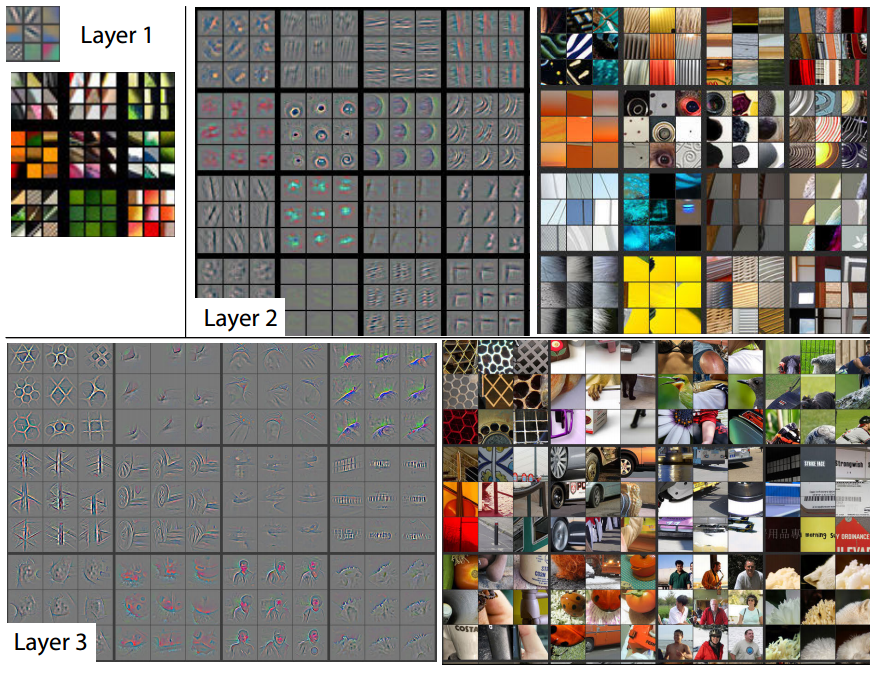
\includegraphics[scale=0.625]{images/filters}
	\caption{Taken from \cite{ZeilerFergus:2013}, this figure shows a selection of features across several layers of a fully trained convolutional network using the visualization technique discussed in section \ref{sec:understanding-convolutional-networks}.}
	\label{fig:feature-activations}
\end{figure}
In the course of this paper we discussed the basic notions of both neural networks in general and the multilayer perceptron in particular. With deep learning in mind, we introduced supervised training using gradient descent and error backropagation as well as unsupervised training using auto encoders. We concluded the section with a brief discussion of regularization methods including dropout \cite{HintonSrivastavaKrizhevskySutskeverSalakhutdinov:2012} and unsupervised pre-training.

We introduced convolutional neural networks by discussing the different types of layers used in recent implementations: the convolutional layer; the non-linearity layer; the rectification layer; the local contrast normalization layer; and the pooling and subsampling layer. Based on these basic building blocks, we discussed the traditional convolutional neural networks \cite{LeCunBoserDenkerHenderson:1989} as well as a modern variant as used in~\cite{KrizhevskySutskeverHinton:2012}.

Despite of their excellent performance \cite{KrizhevskySutskeverHinton:2012, CiresanMeierSchmidhuber:2012}, the internal operation of convolutional neural networks is not well understood \cite{ZeilerFergus:2013}. To get deeper insight into their internal working, we followed \cite{ZeilerFergus:2013} and discussed a visualization technique allowing to backproject the feature activations of higher layers. This allows to further evaluate and improve recent architectures as for example the architecture used in \cite{KrizhevskySutskeverHinton:2012}.

Nevertheless, convolutional neural networks and deep learning in general is an active area of research. Although the difficulty of deep learning seems to be understood \cite{Bengio:2009,GlorotBengio:2010,ErhanManzagolBengioVincent:2009}, learning feature hierarchies is considered very hard \cite{Bengio:2009}. Here, the possibility of unsupervised pre-training had a huge impact and allows to train deep architectures in reasonable time \cite{Bengio:2009,ErhanBengioCourvilleManzagolVincentBengio:2010}. Nonetheless, the reason for the good performance of deep neural networks is still not answered fully.

% The different layers present in recent convolutional networks were introduced in section three. Based on these basic building blocks, we discussed the traditional convolutional neural networks as proposed in \cite{LeCunBoserDenkerHenderson:1989} as well as a more recent implementation as described in \cite{KrizhevskySutskeverHinton:2012}.

% Based on the deconvolutional neural networks, as introduced in \cite{ZeilerKrishnanTaylorFergus:2010}, the authors of \cite{ZeilerFergus:2013} propose a visualization technique allowing to backproject feature activations of higher layers onto the image plain. This allows to get deeper insights into the operation of deep convolutional neural networks.

% Still, training deep architectures is considered a challenge in machine learning \cite{Bengio:2009}. Although, convolutional neural networks can be seen as exception -- as deep convolutional networks are more easily trained due to their constrained architecture --, understanding deep learning is currently a promising research area. In addition, deep architectures allow to learn complex, task specific features (SOURCE) where they would have been handcrafted before. 

% In 2006, the work in \cite{HintonOsindero:2006} is considered as breakthrough in deep learning, as it allows to pre-train deep networks in an unsupervised fashion. Using unsupervised pre-training, deep networks can be trained with traditional methods as gradient descent and the error backpropagation algorithm.

% Nevertheless, the internal operation of higher layers in both convolutional networks as well as general neural networks are not well understood. Here, the work in \cite{ZeilerFergus:2013} allows to visualize feature activations of higher layers and, thus, allows to get more insight into the internal operations. Based on the visualization, architectures can be adapted to give better performance or generalization as well as better training speed.

	\bibliographystyle{alpha}
	\bibliography{seminar}
\end{document}
